\chapter{Różnica długości członów a pozycja krótszego członu} \label{dod:wykresy}
\graphicspath{{results/plots}}

\section{Języki inicjalne}

\begin{sidewaysfigure}
\centering
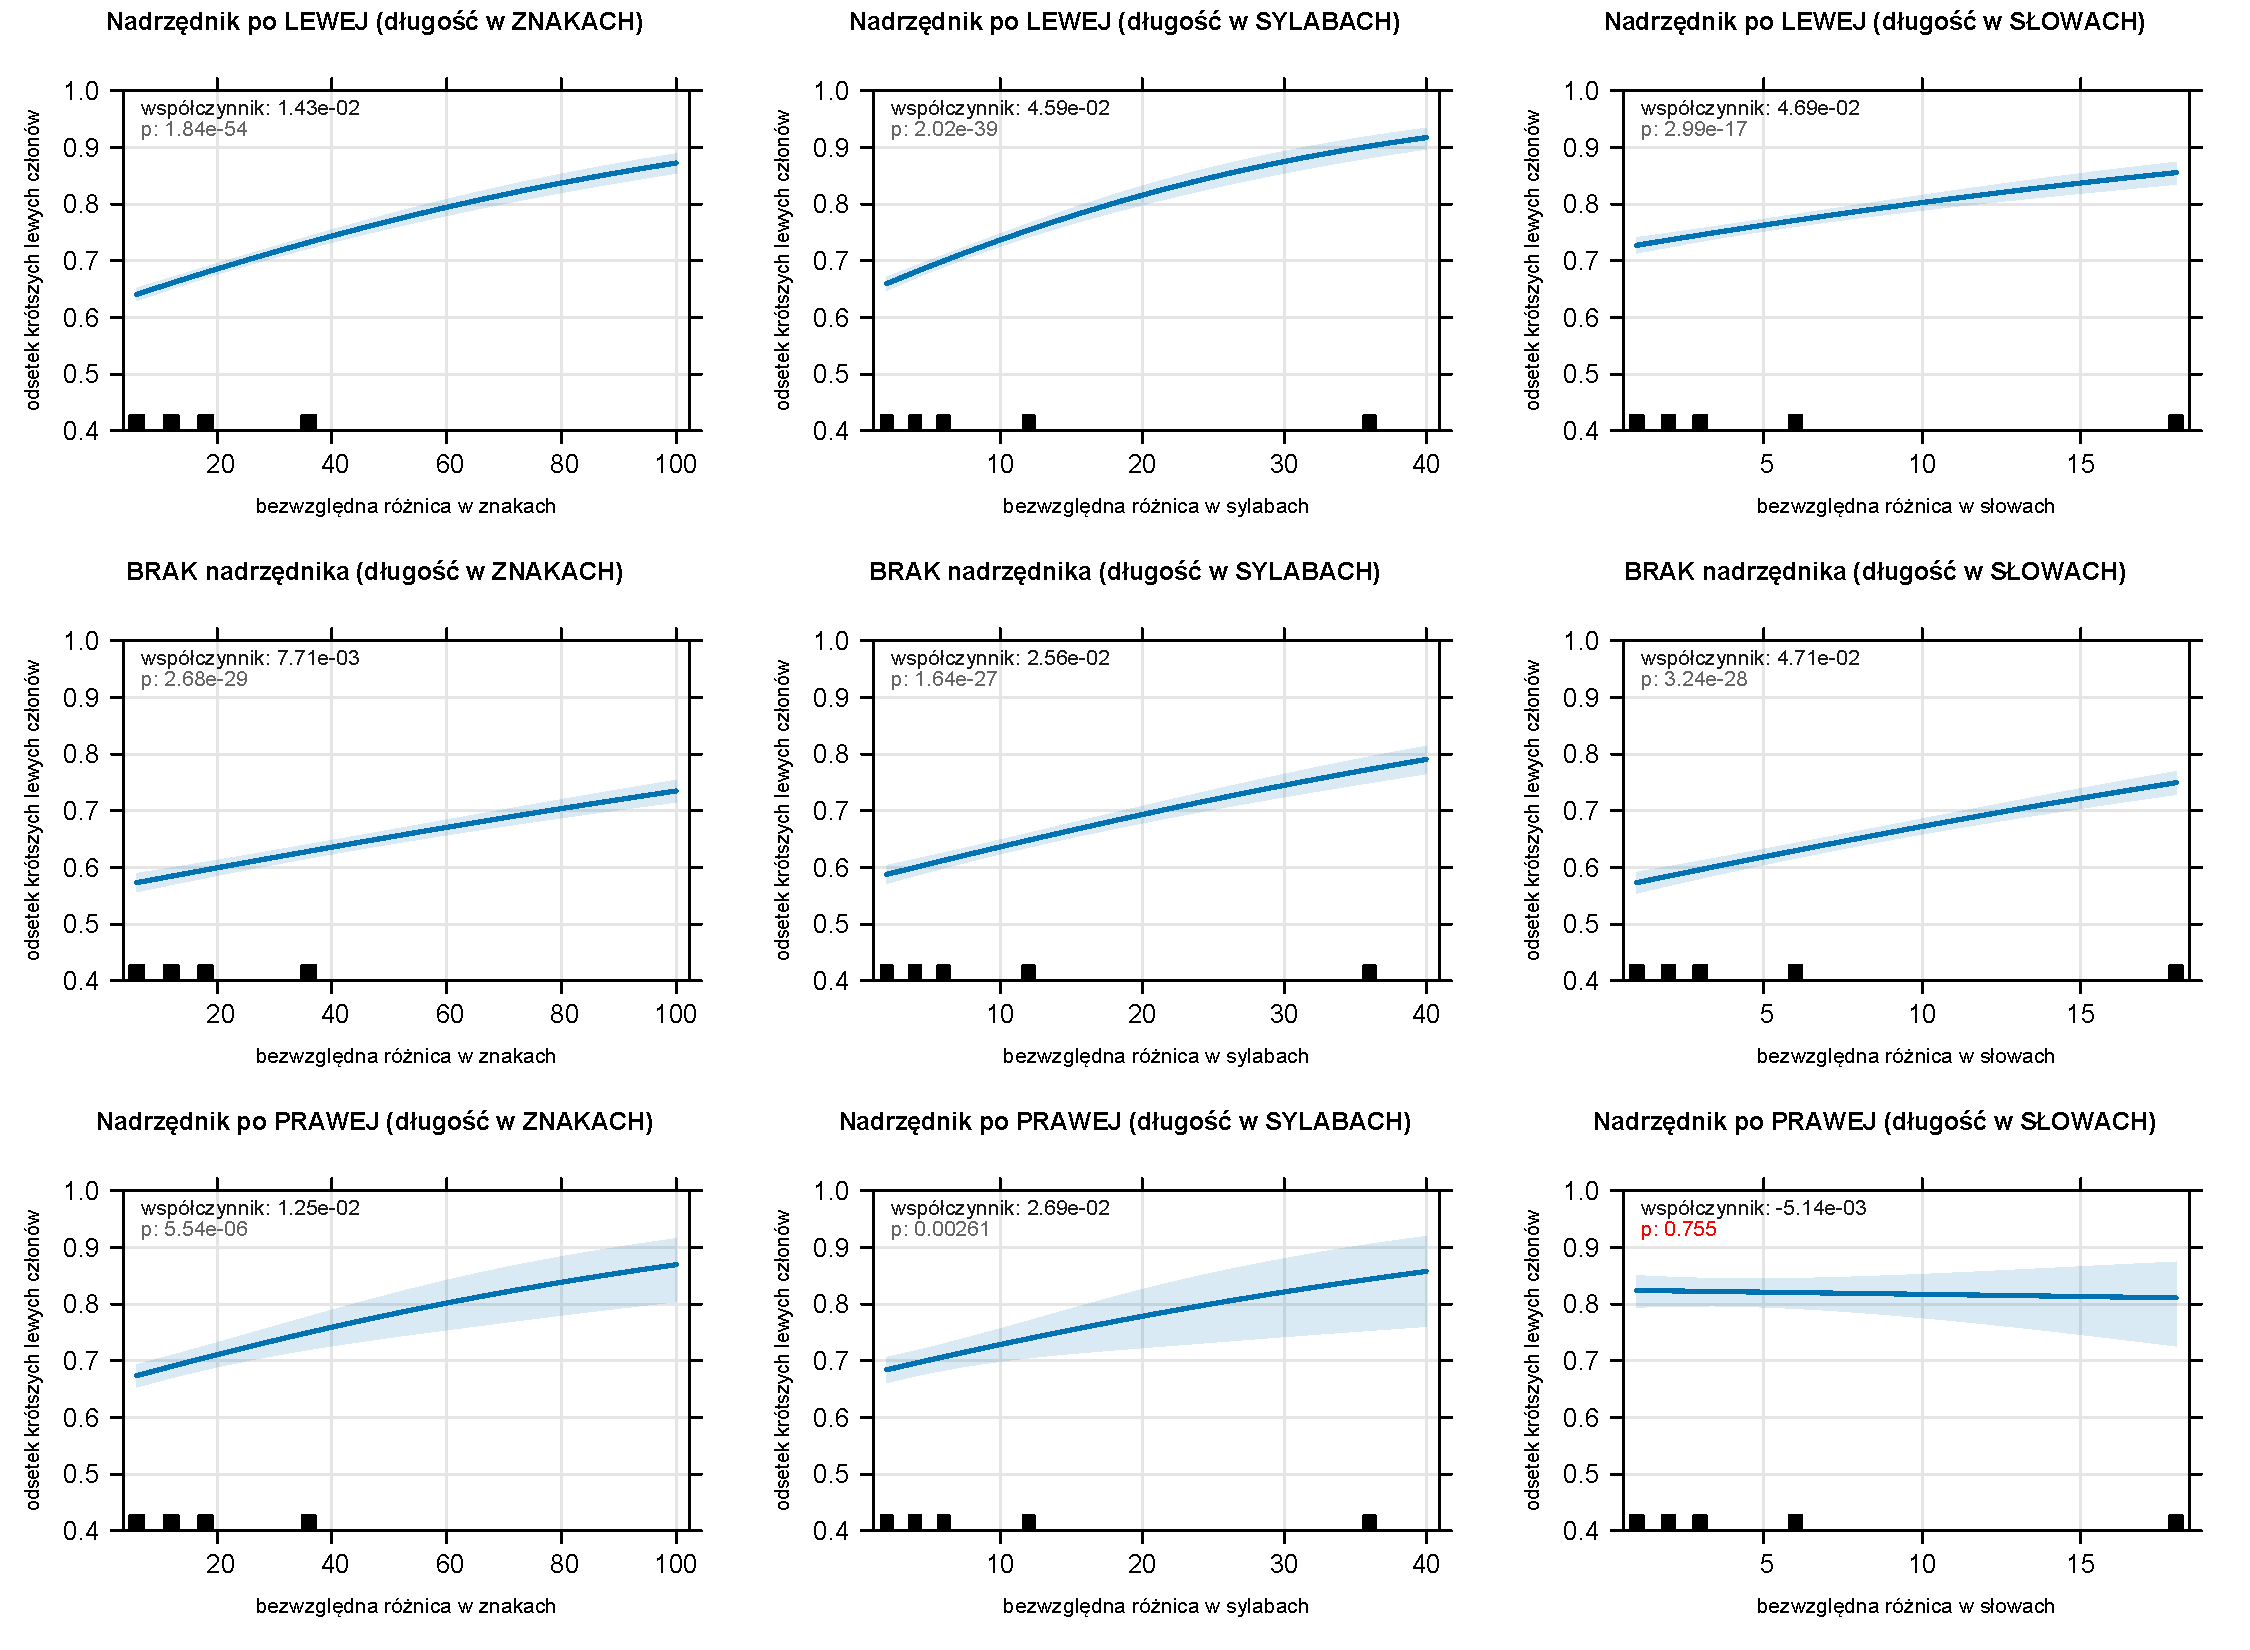
\includegraphics[scale=0.6]{English.pdf}
\caption{Różnica długości członów a występowanie krótszego członu po lewej stronie -- język \textbf{angielski}}
\label{fig:en}
\end{sidewaysfigure}

\begin{sidewaysfigure}
\centering
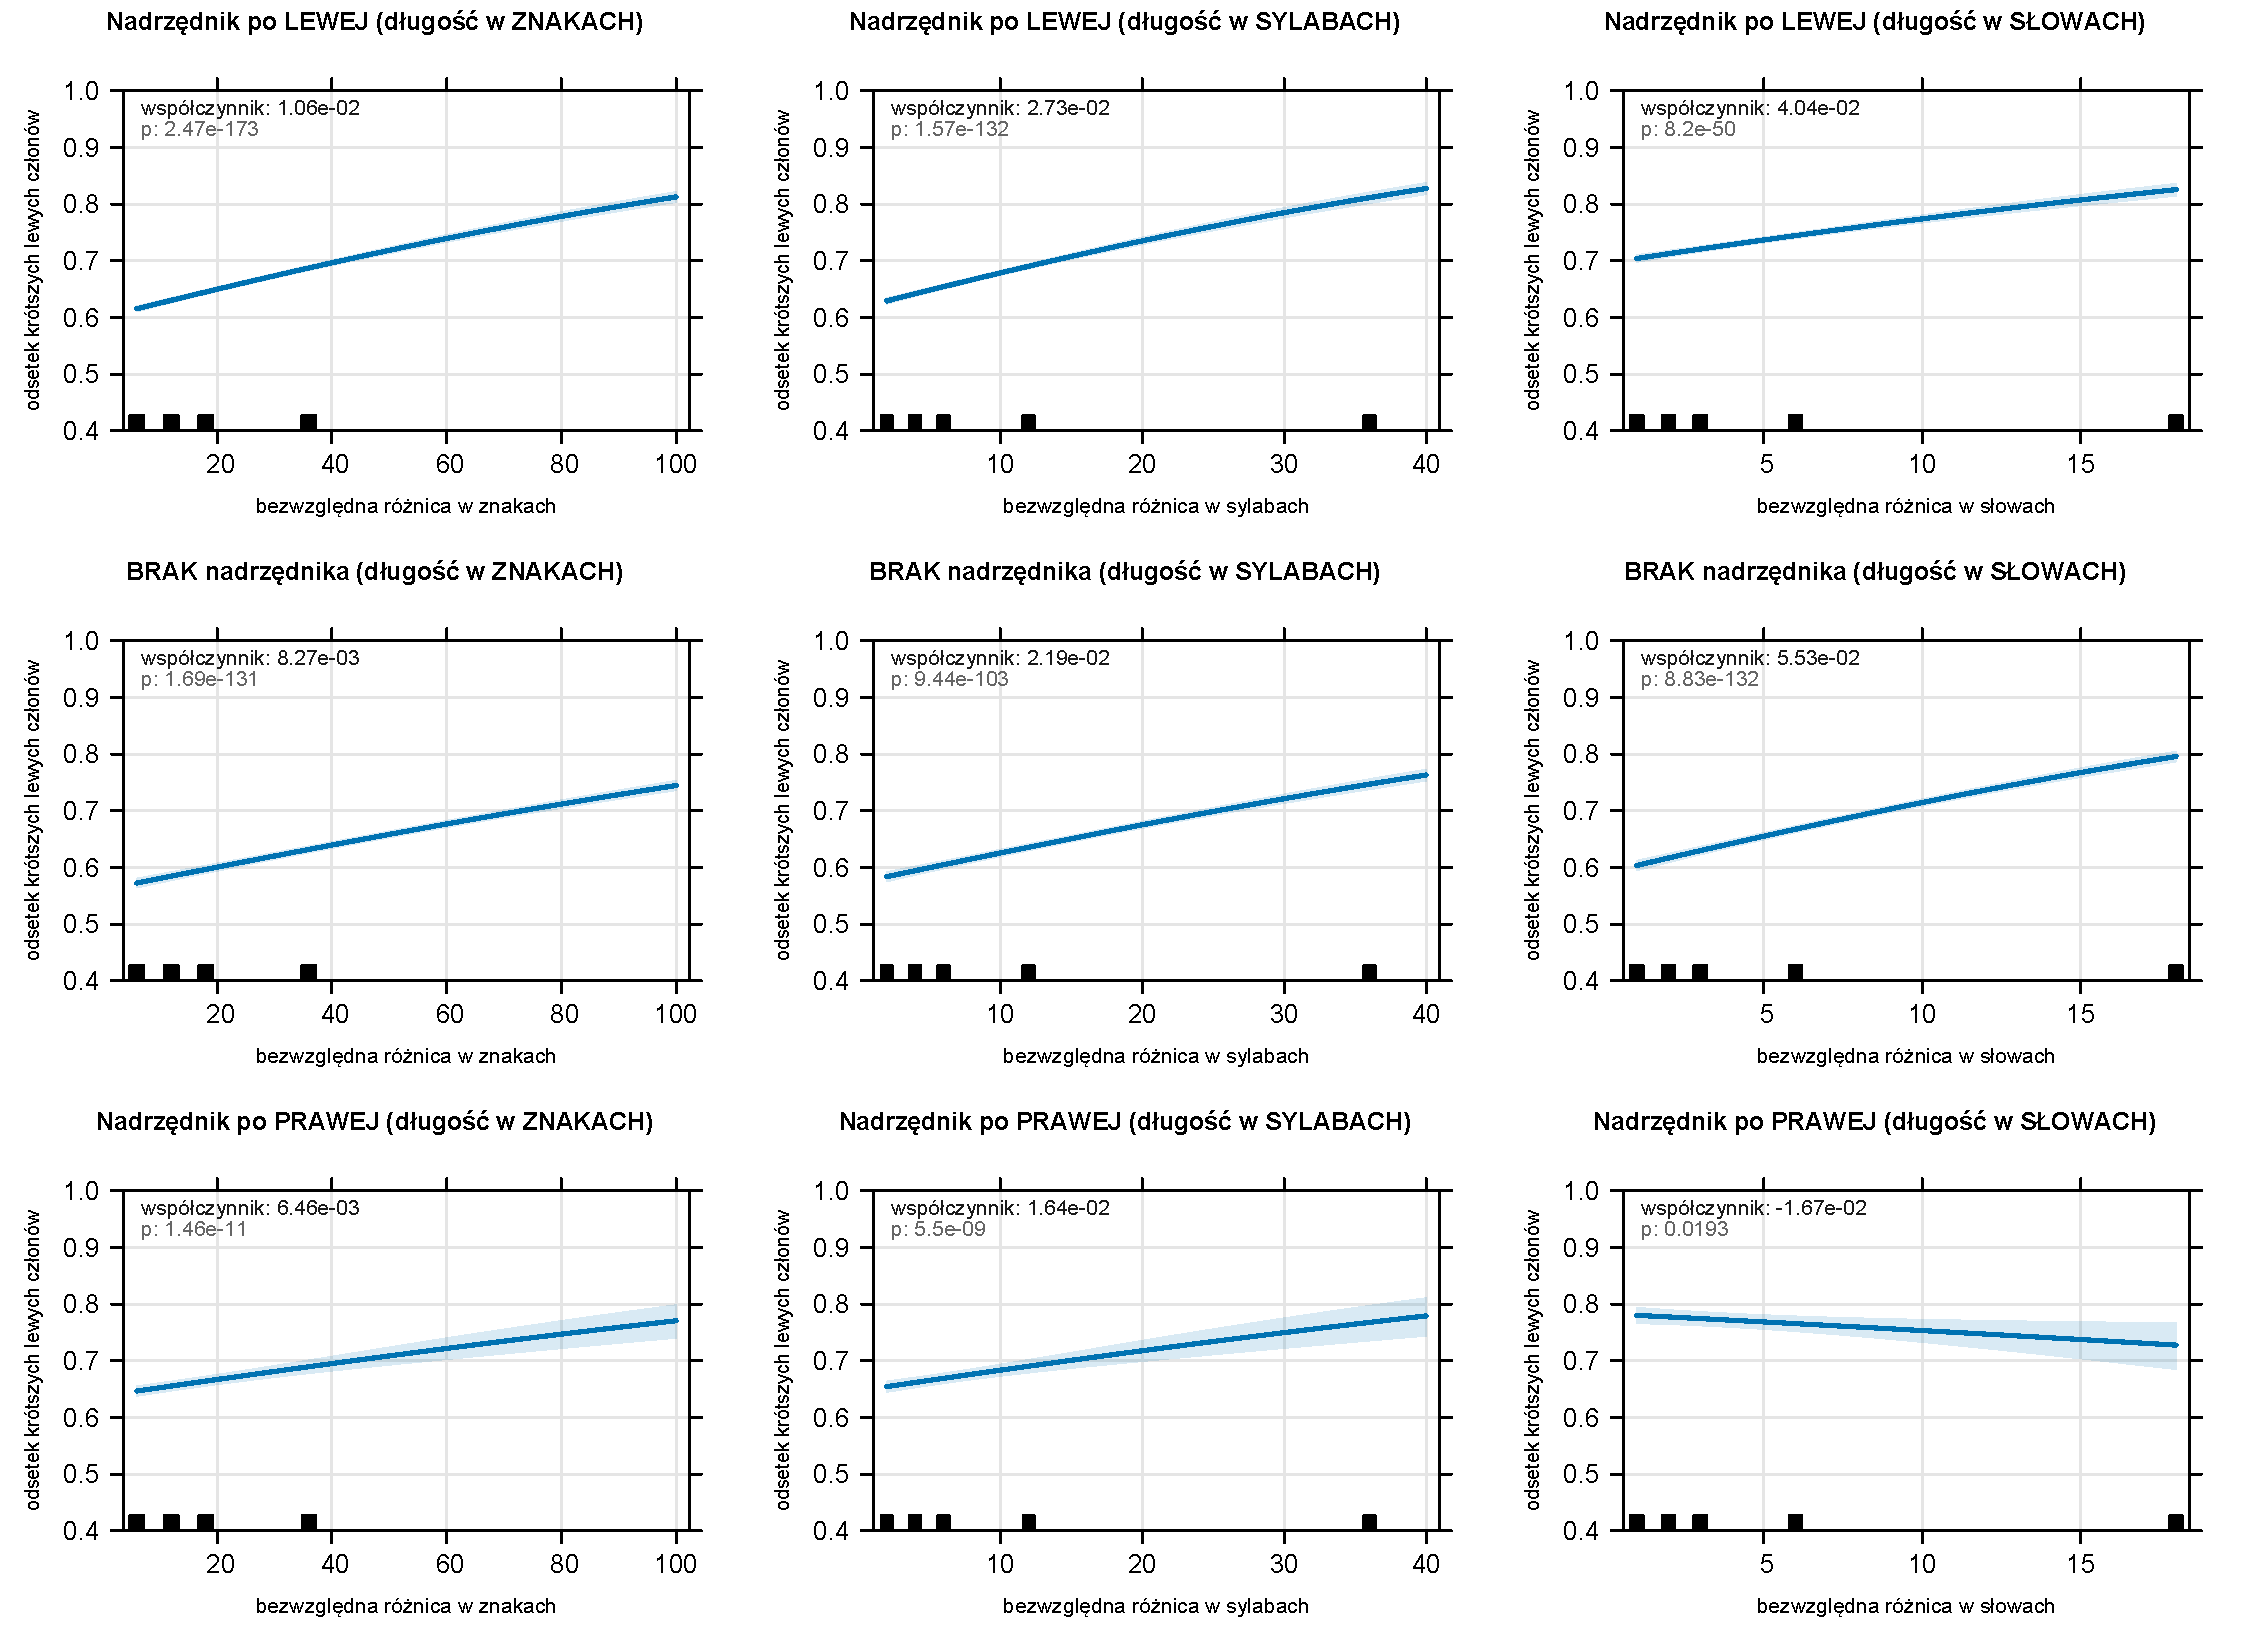
\includegraphics[scale=0.6]{Czech.pdf}
\caption{Różnica długości członów a występowanie krótszego członu po lewej stronie -- język \textbf{czeski}}
\label{fig:cz}
\end{sidewaysfigure}

\begin{sidewaysfigure}
\centering
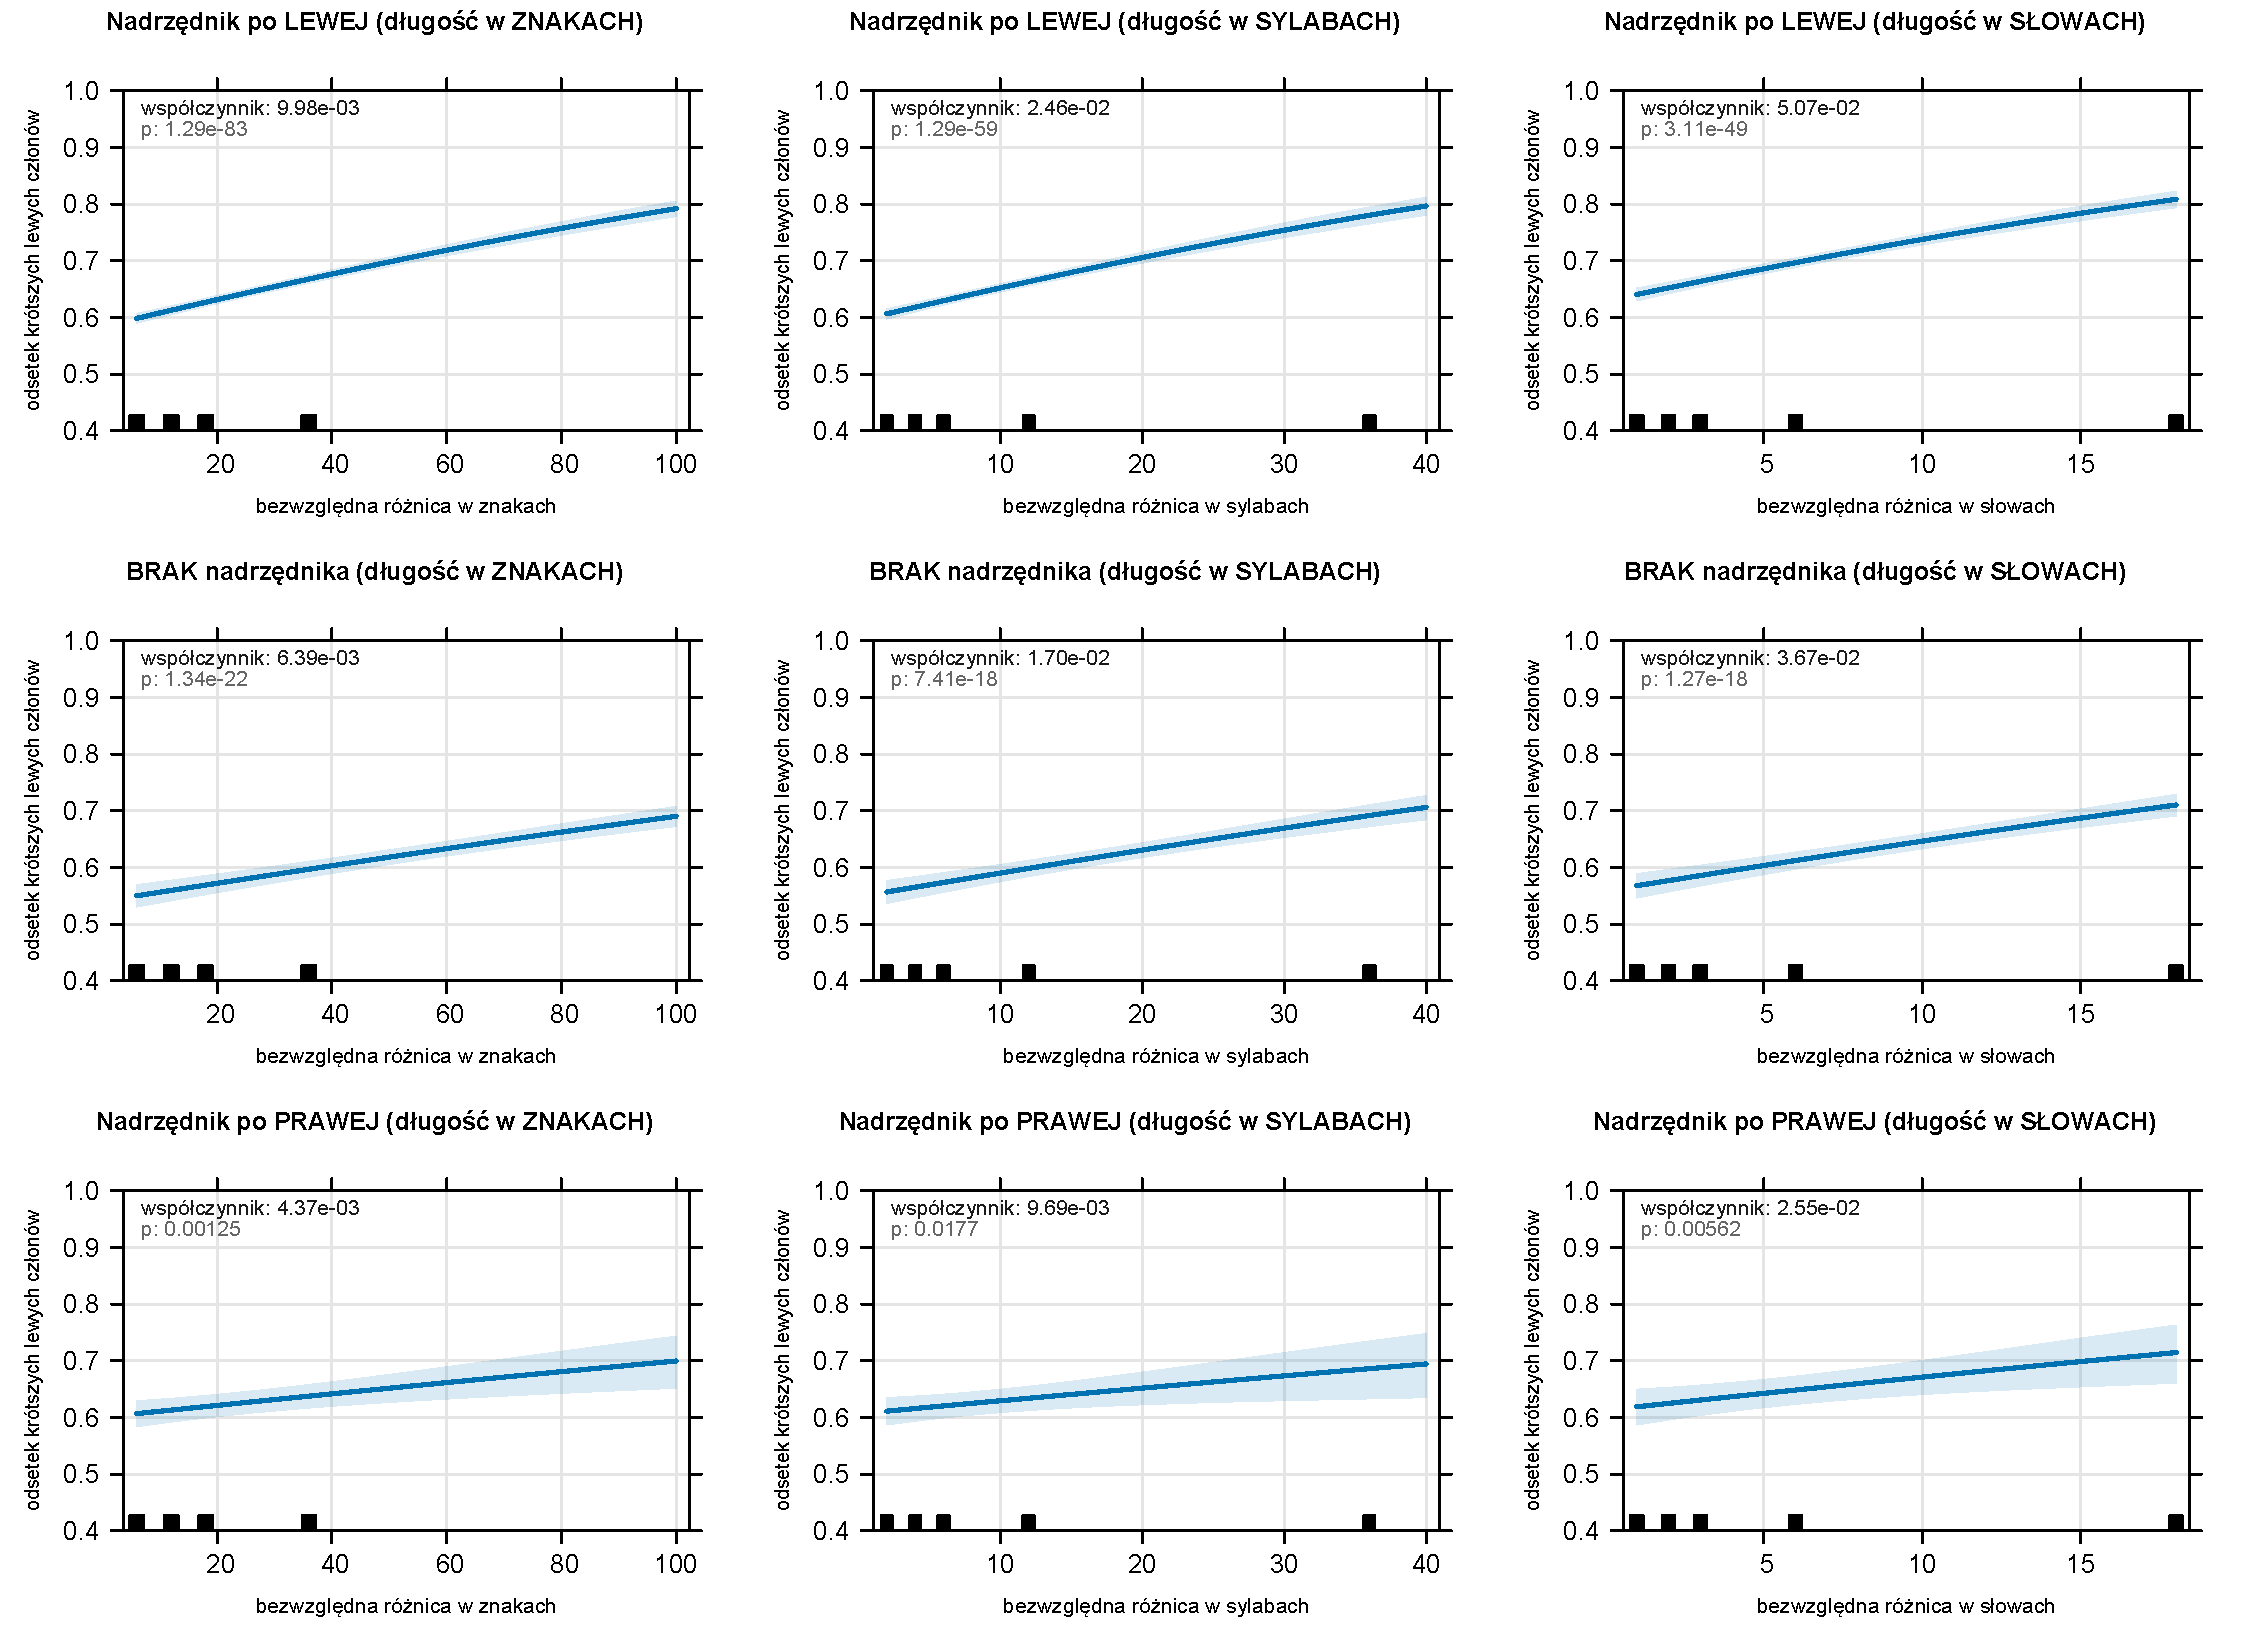
\includegraphics[scale=0.6]{Spanish.pdf}
\caption{Różnica długości członów a występowanie krótszego członu po lewej stronie -- język \textbf{hiszpański}}
\label{fig:es}
\end{sidewaysfigure}

\begin{sidewaysfigure}
\centering
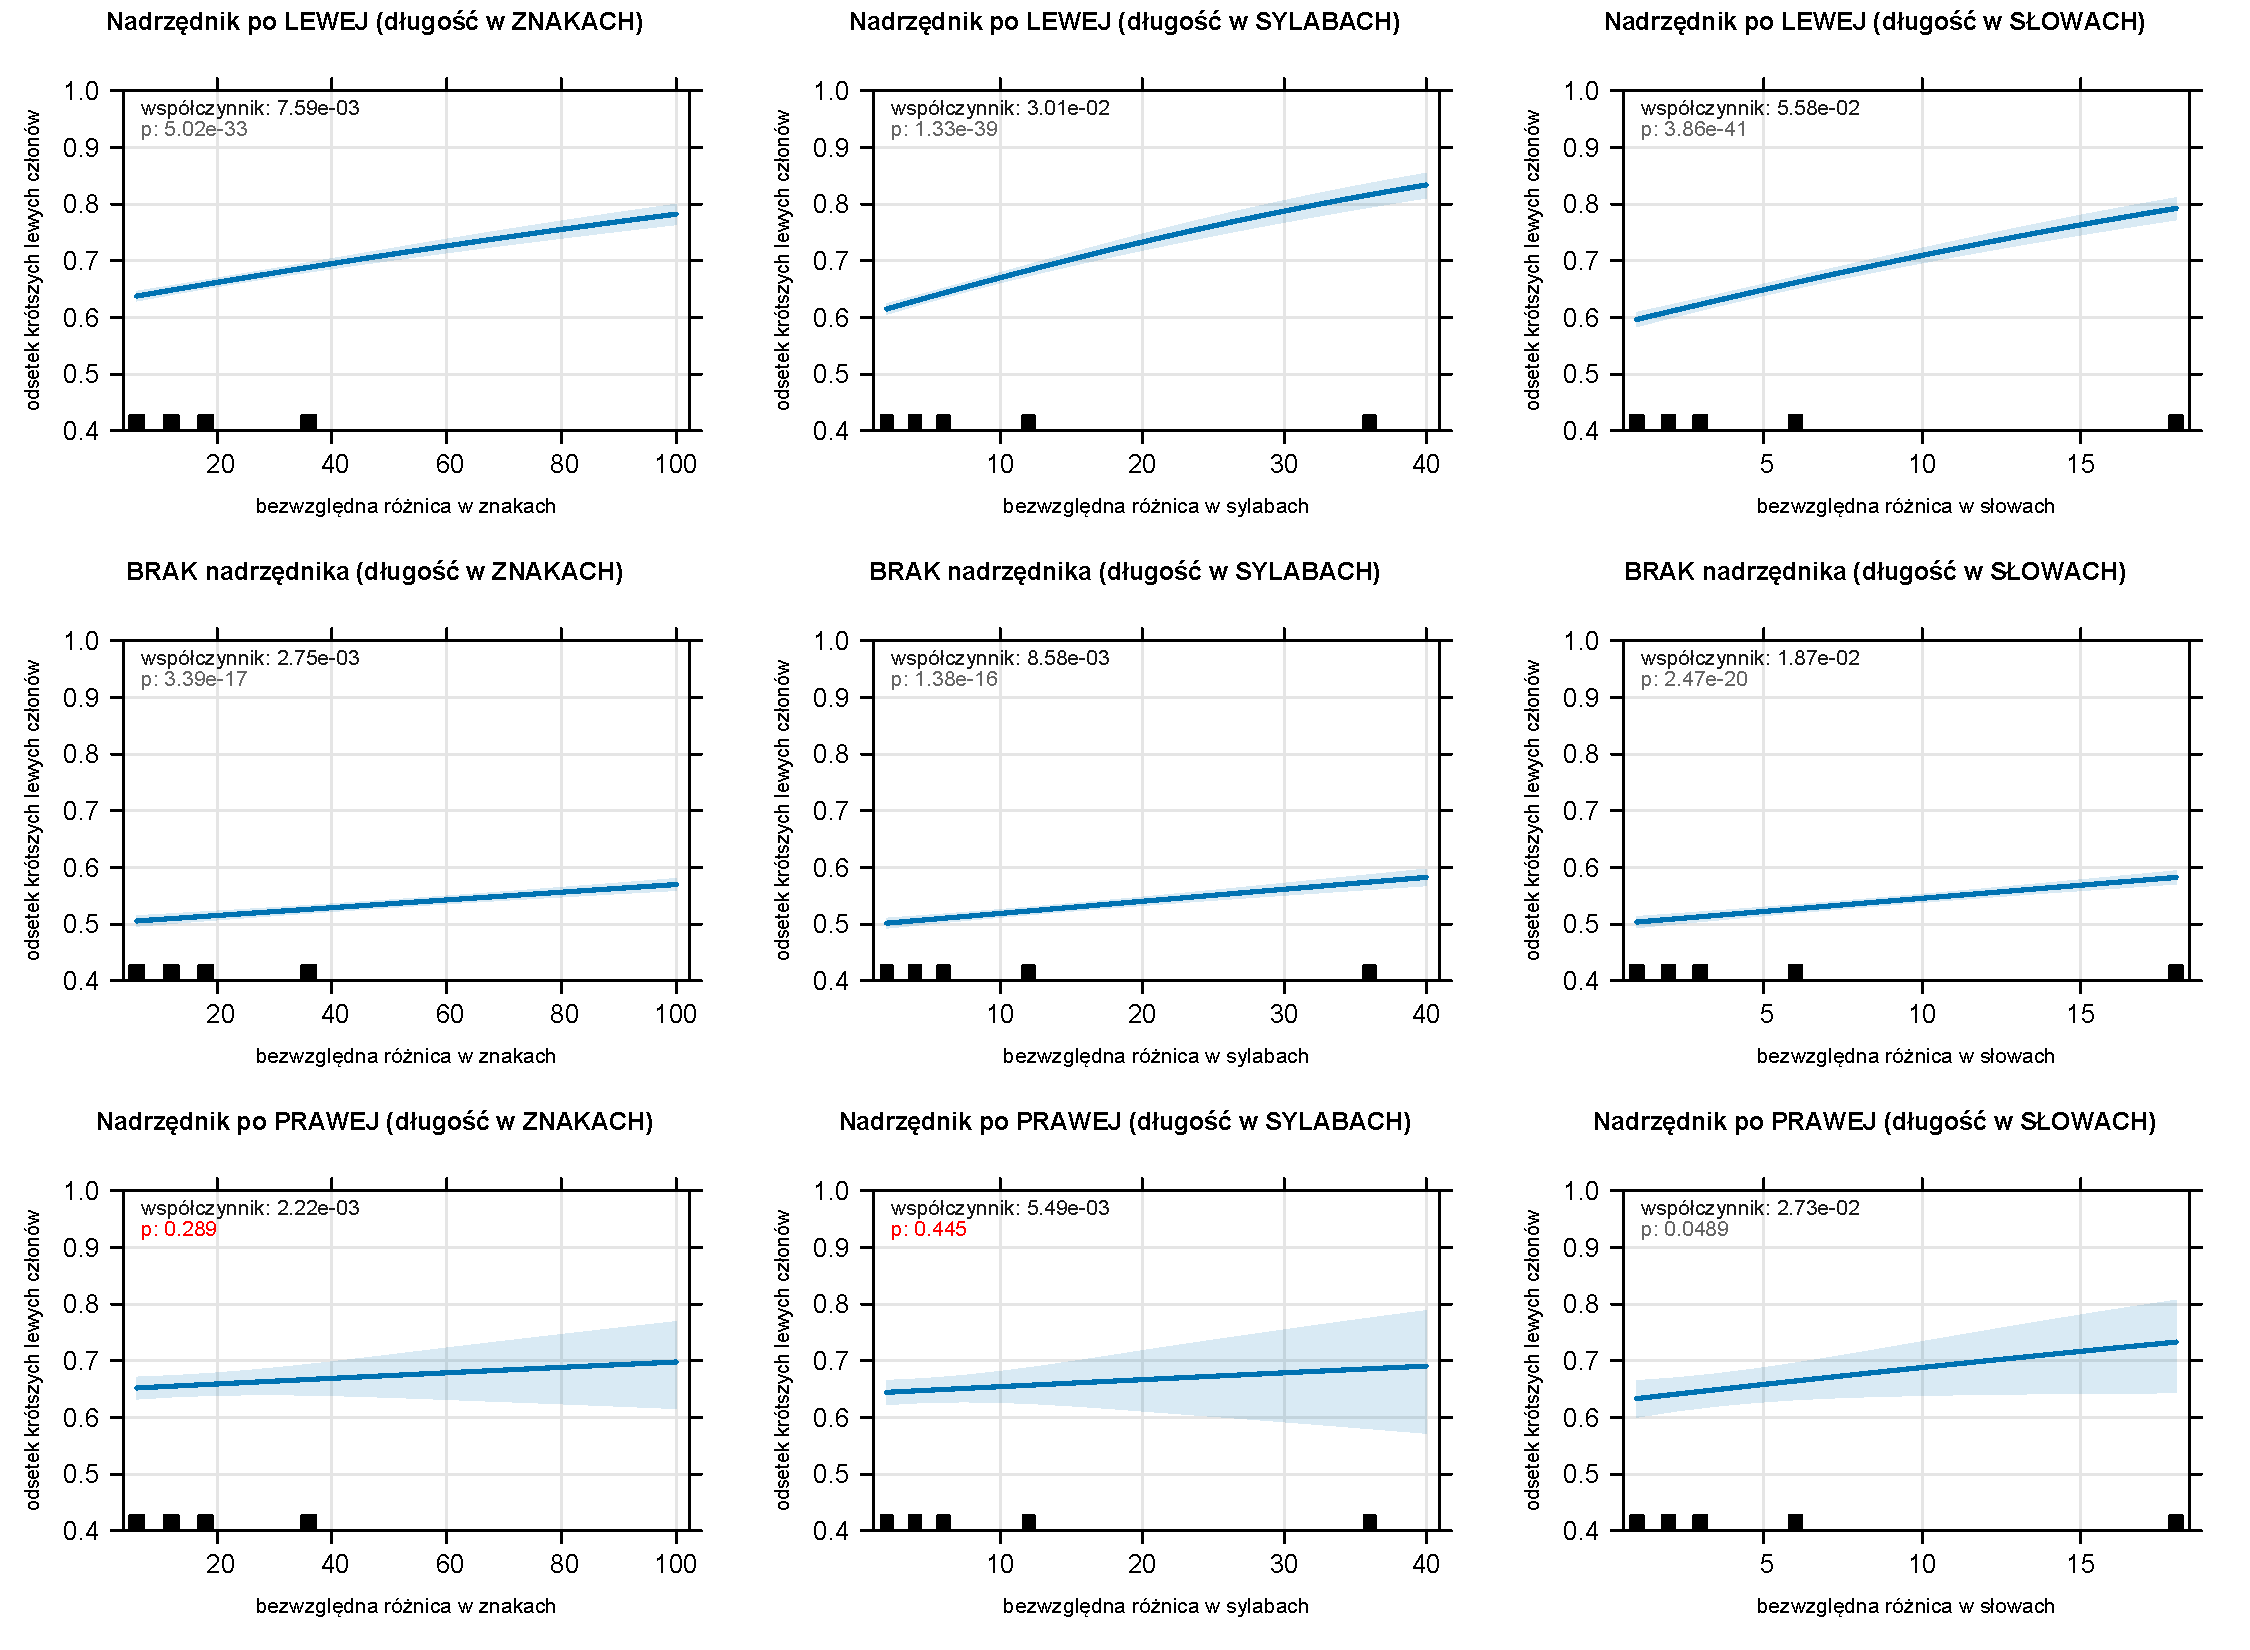
\includegraphics[scale=0.6]{Icelandic.pdf}
\caption{Różnica długości członów a występowanie krótszego członu po lewej stronie -- język \textbf{islandzki}}
\label{fig:is}
\end{sidewaysfigure}

\begin{sidewaysfigure}
\centering
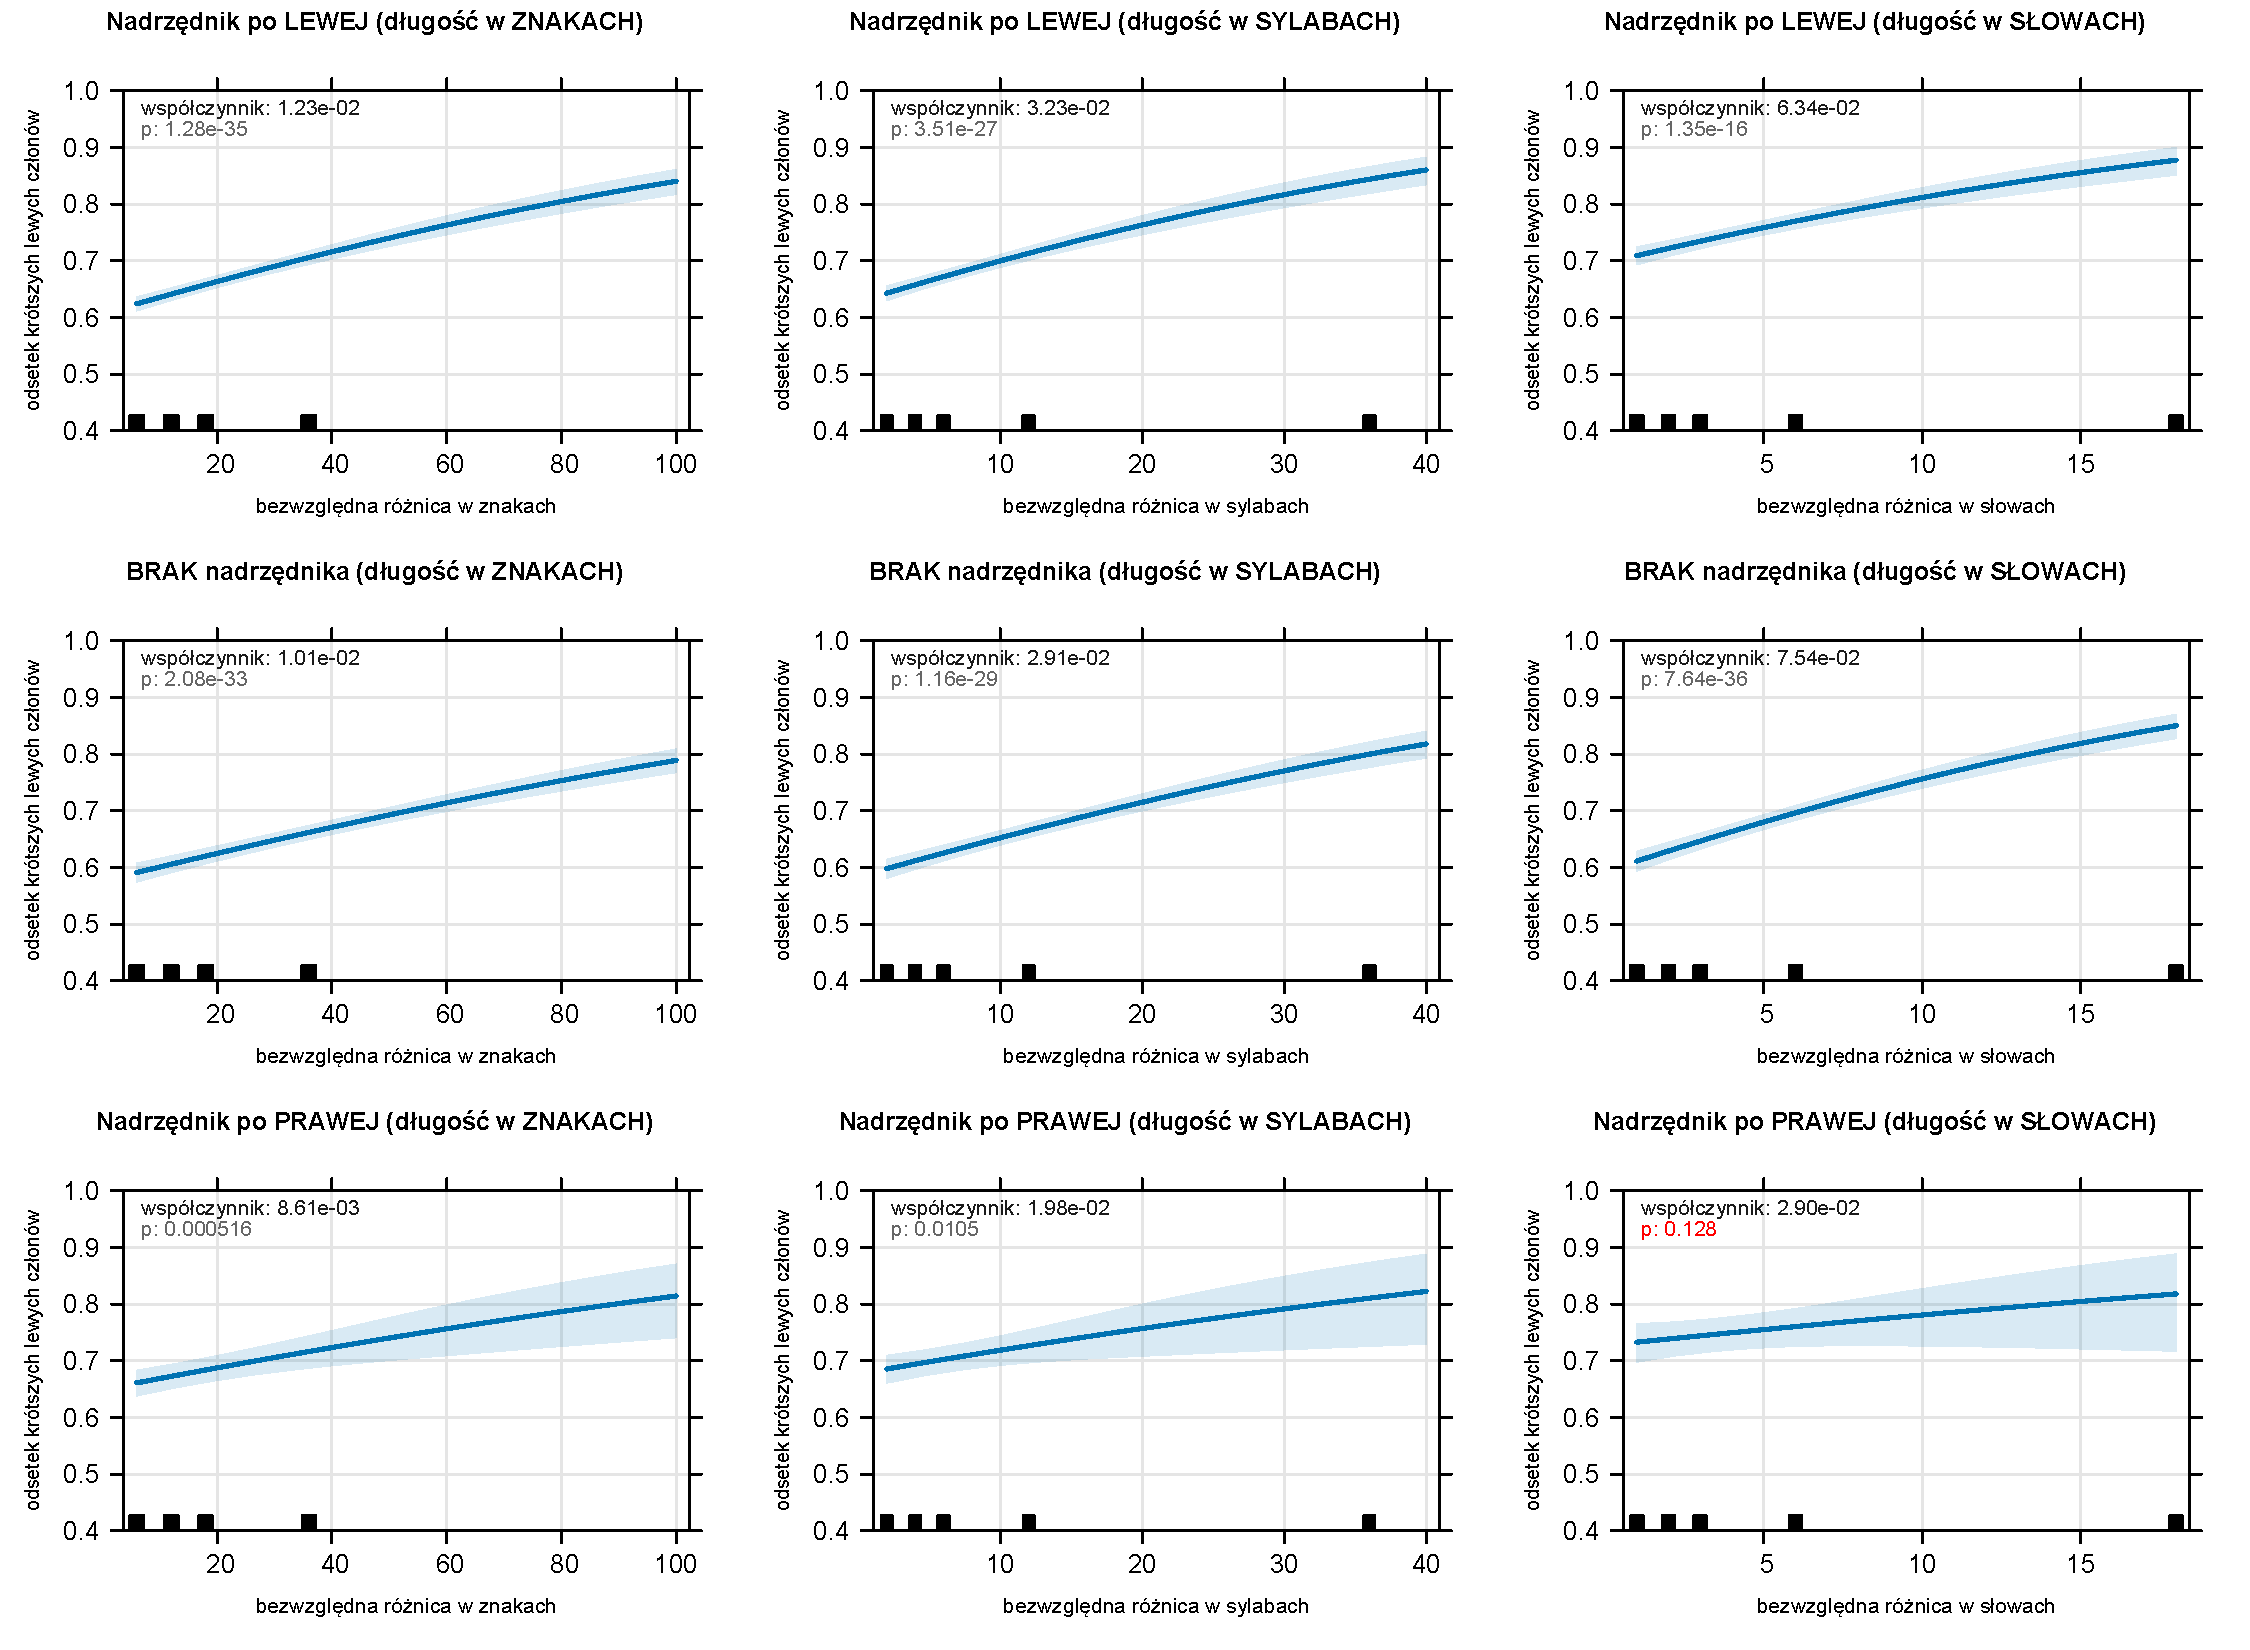
\includegraphics[scale=0.6]{Polish.pdf}
\caption{Różnica długości członów a występowanie krótszego członu po lewej stronie -- język \textbf{polski}}
\label{fig:pl}
\end{sidewaysfigure}

\begin{sidewaysfigure}
\centering
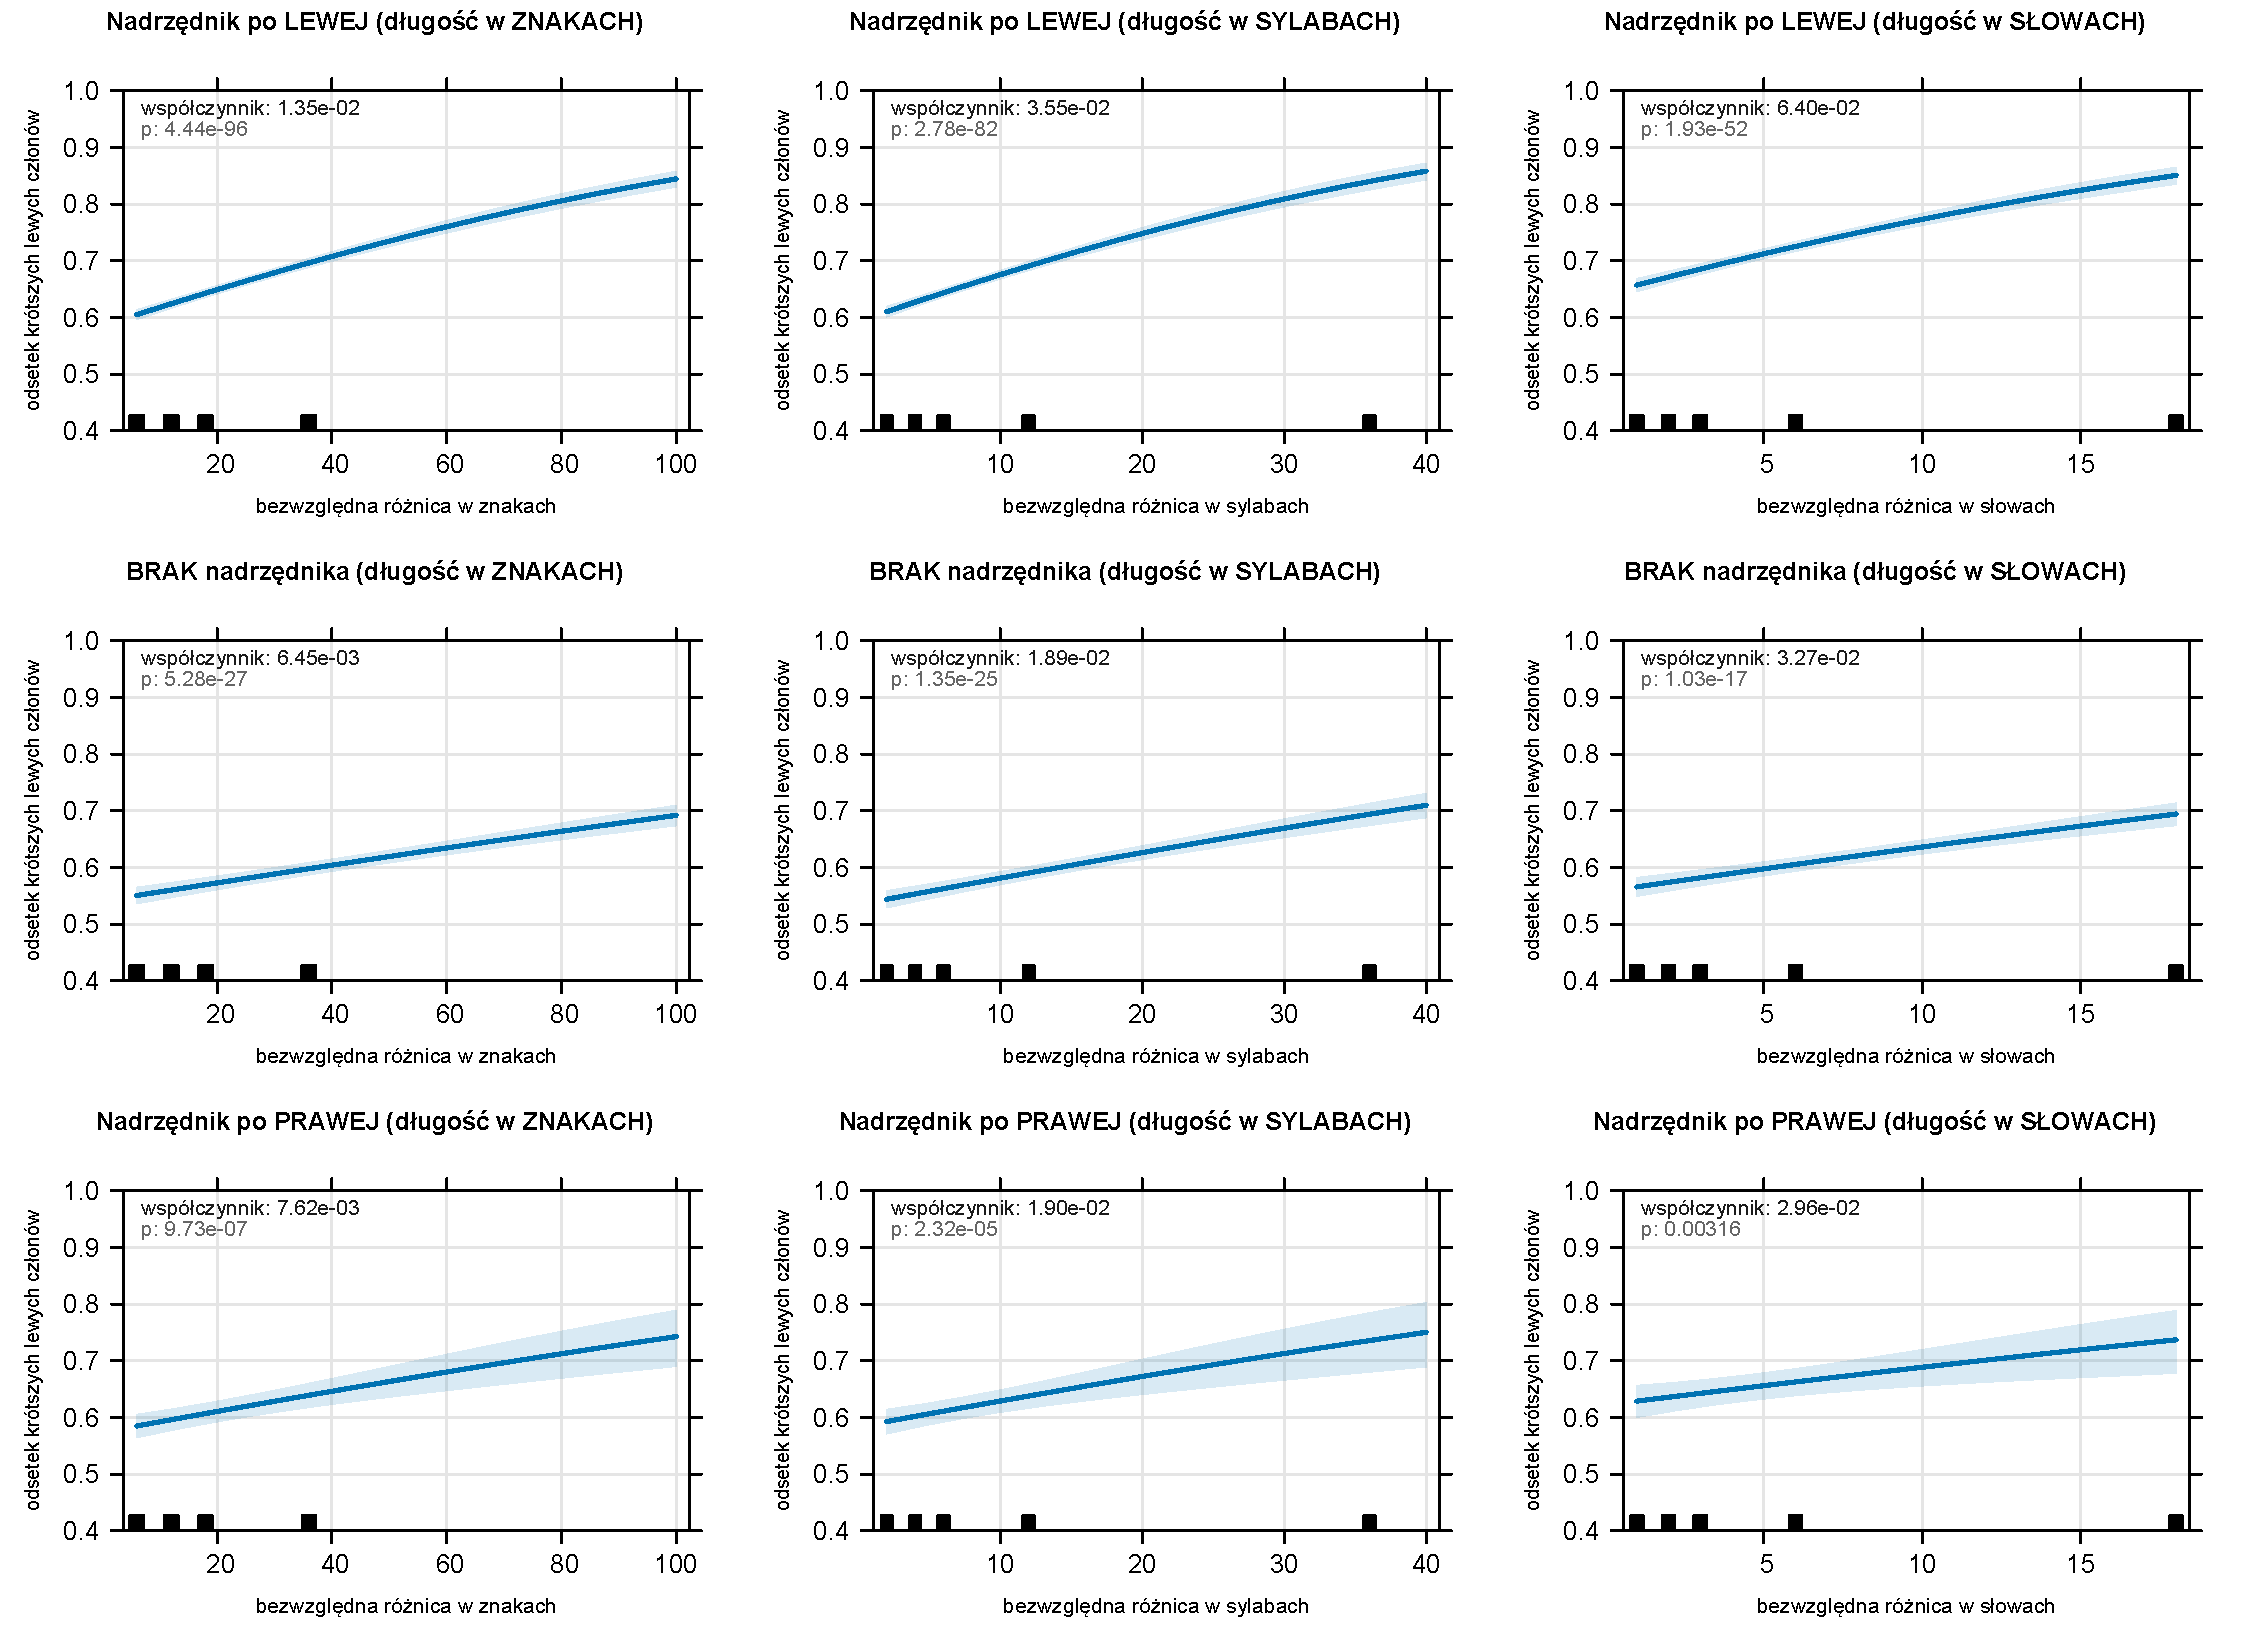
\includegraphics[scale=0.6]{Portuguese.pdf}
\caption{Różnica długości członów a występowanie krótszego członu po lewej stronie -- język \textbf{portugalski}}
\label{fig:po}
\end{sidewaysfigure}

\begin{sidewaysfigure}
\centering
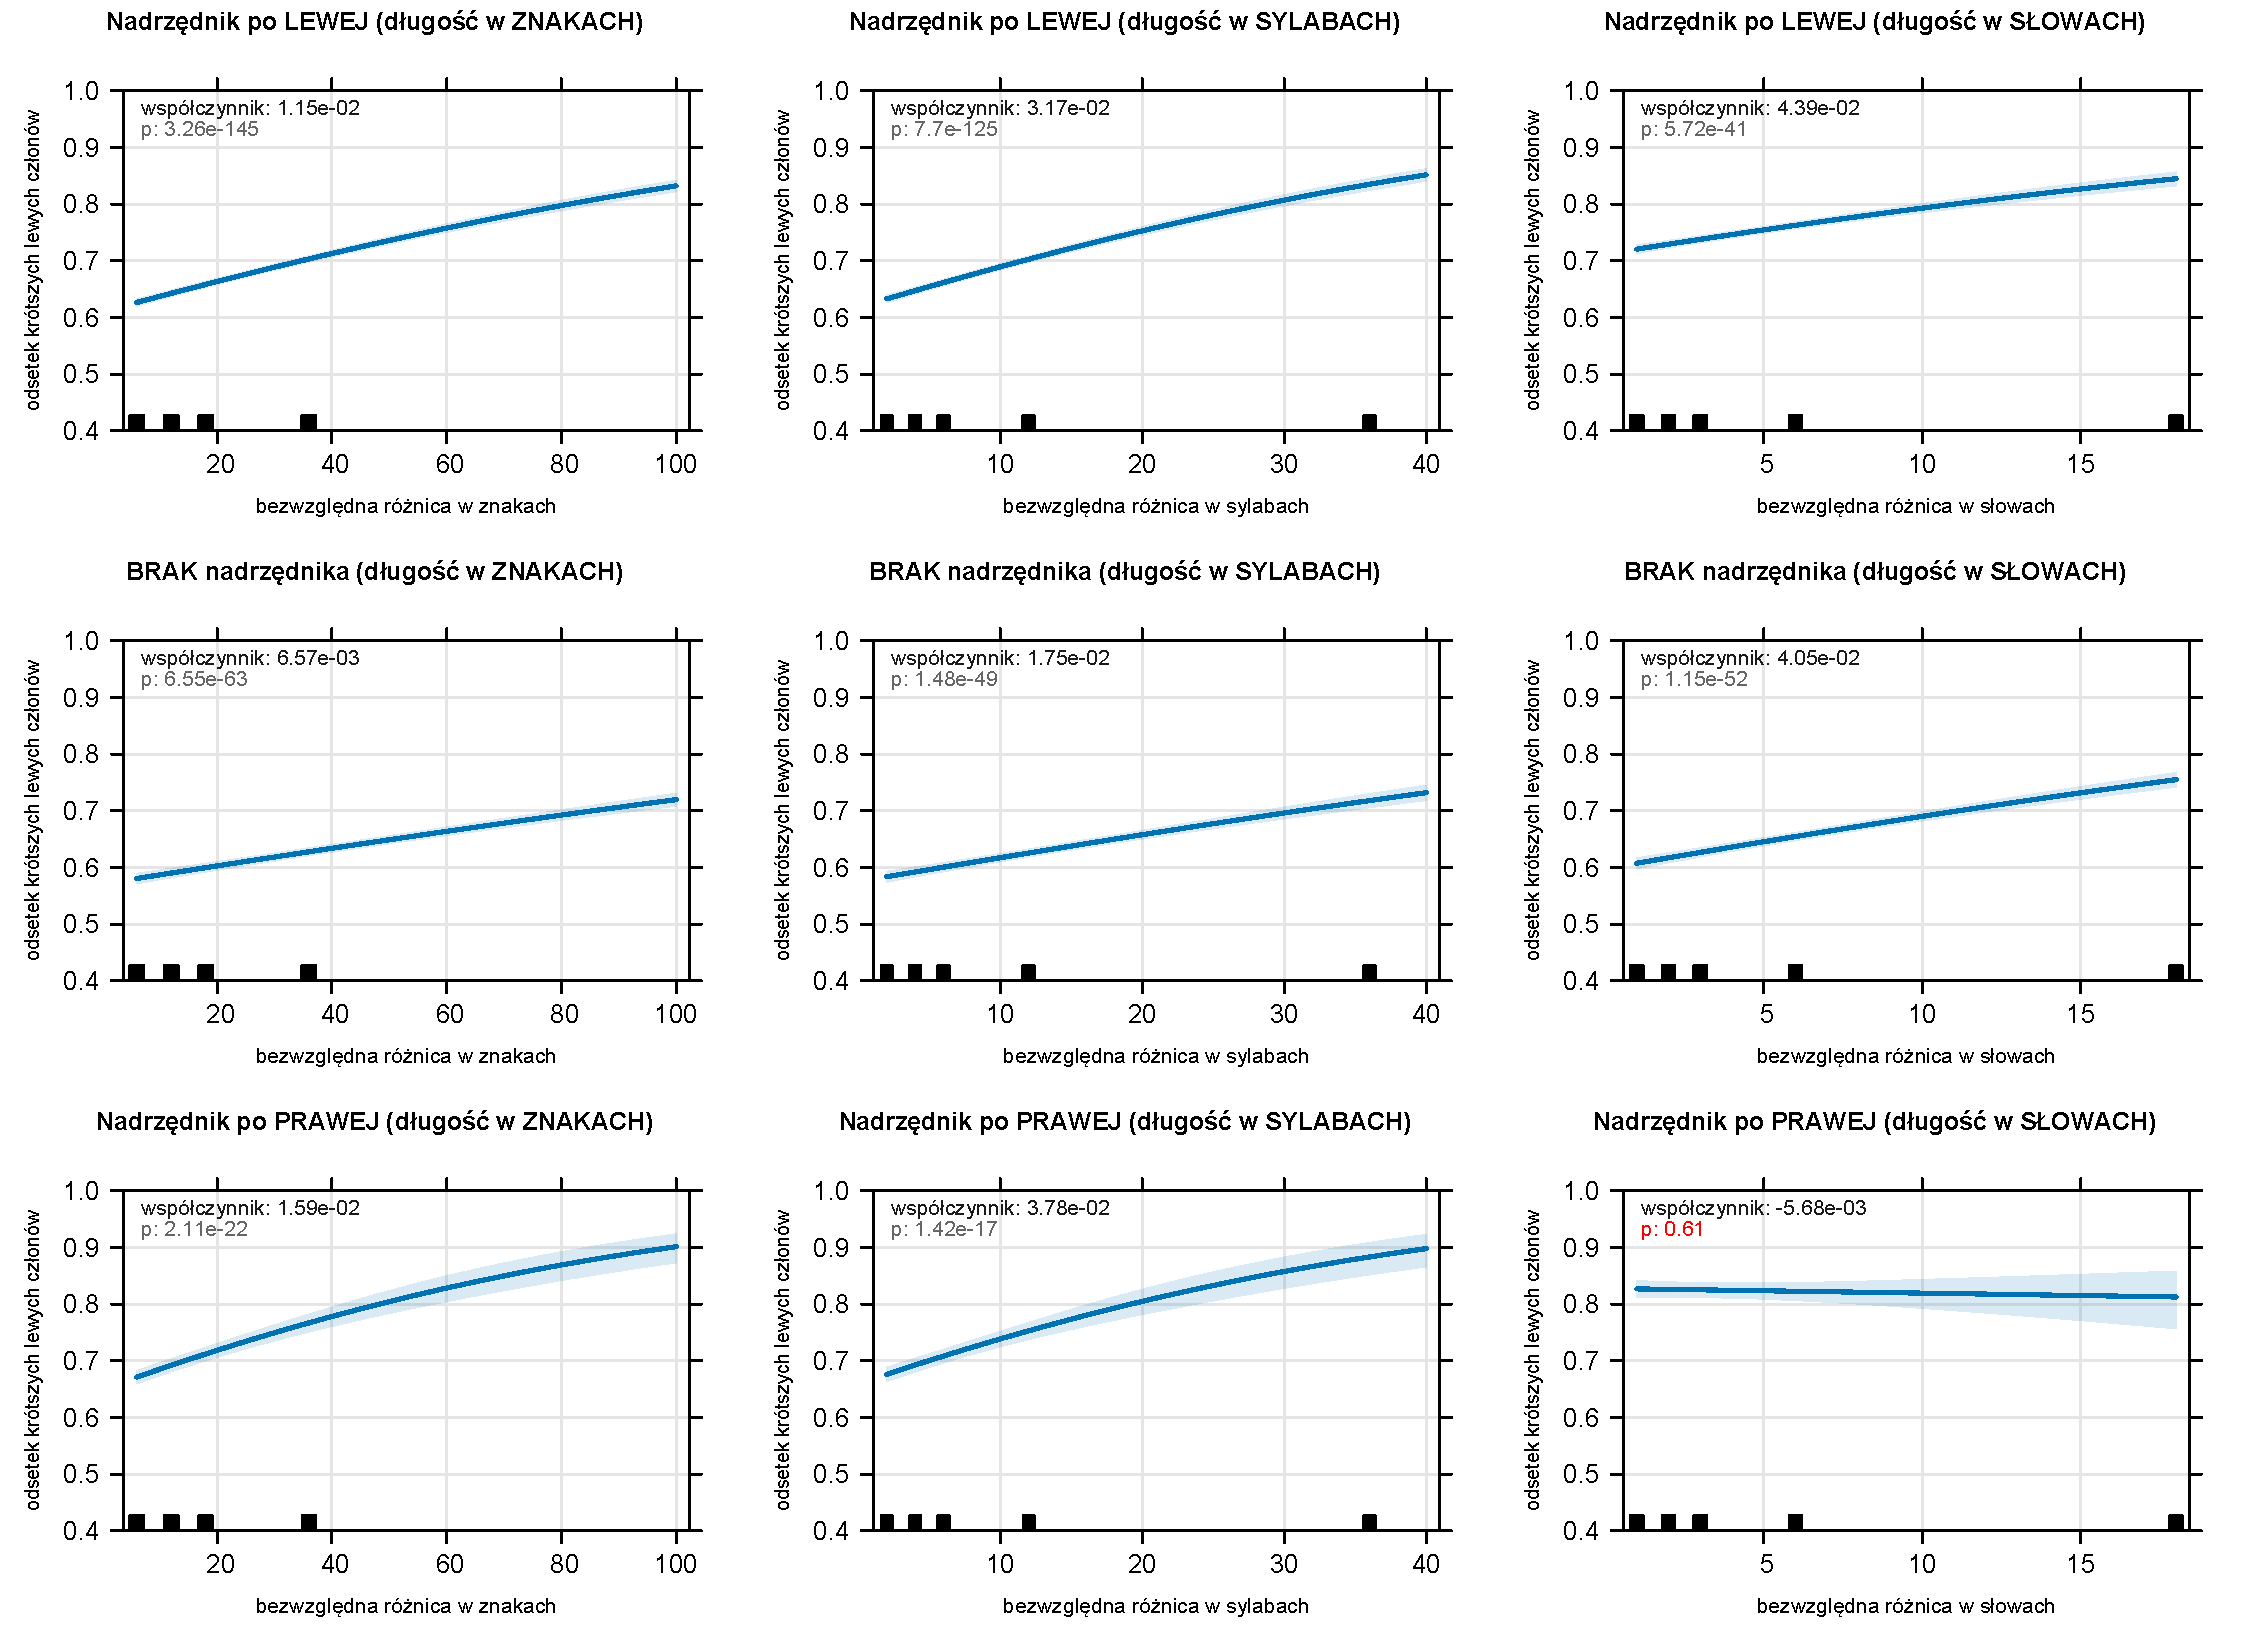
\includegraphics[scale=0.6]{Russian.pdf}
\caption{Różnica długości członów a występowanie krótszego członu po lewej stronie -- język \textbf{rosyjski}}
\label{fig:ru}
\end{sidewaysfigure}

\begin{sidewaysfigure}
\centering
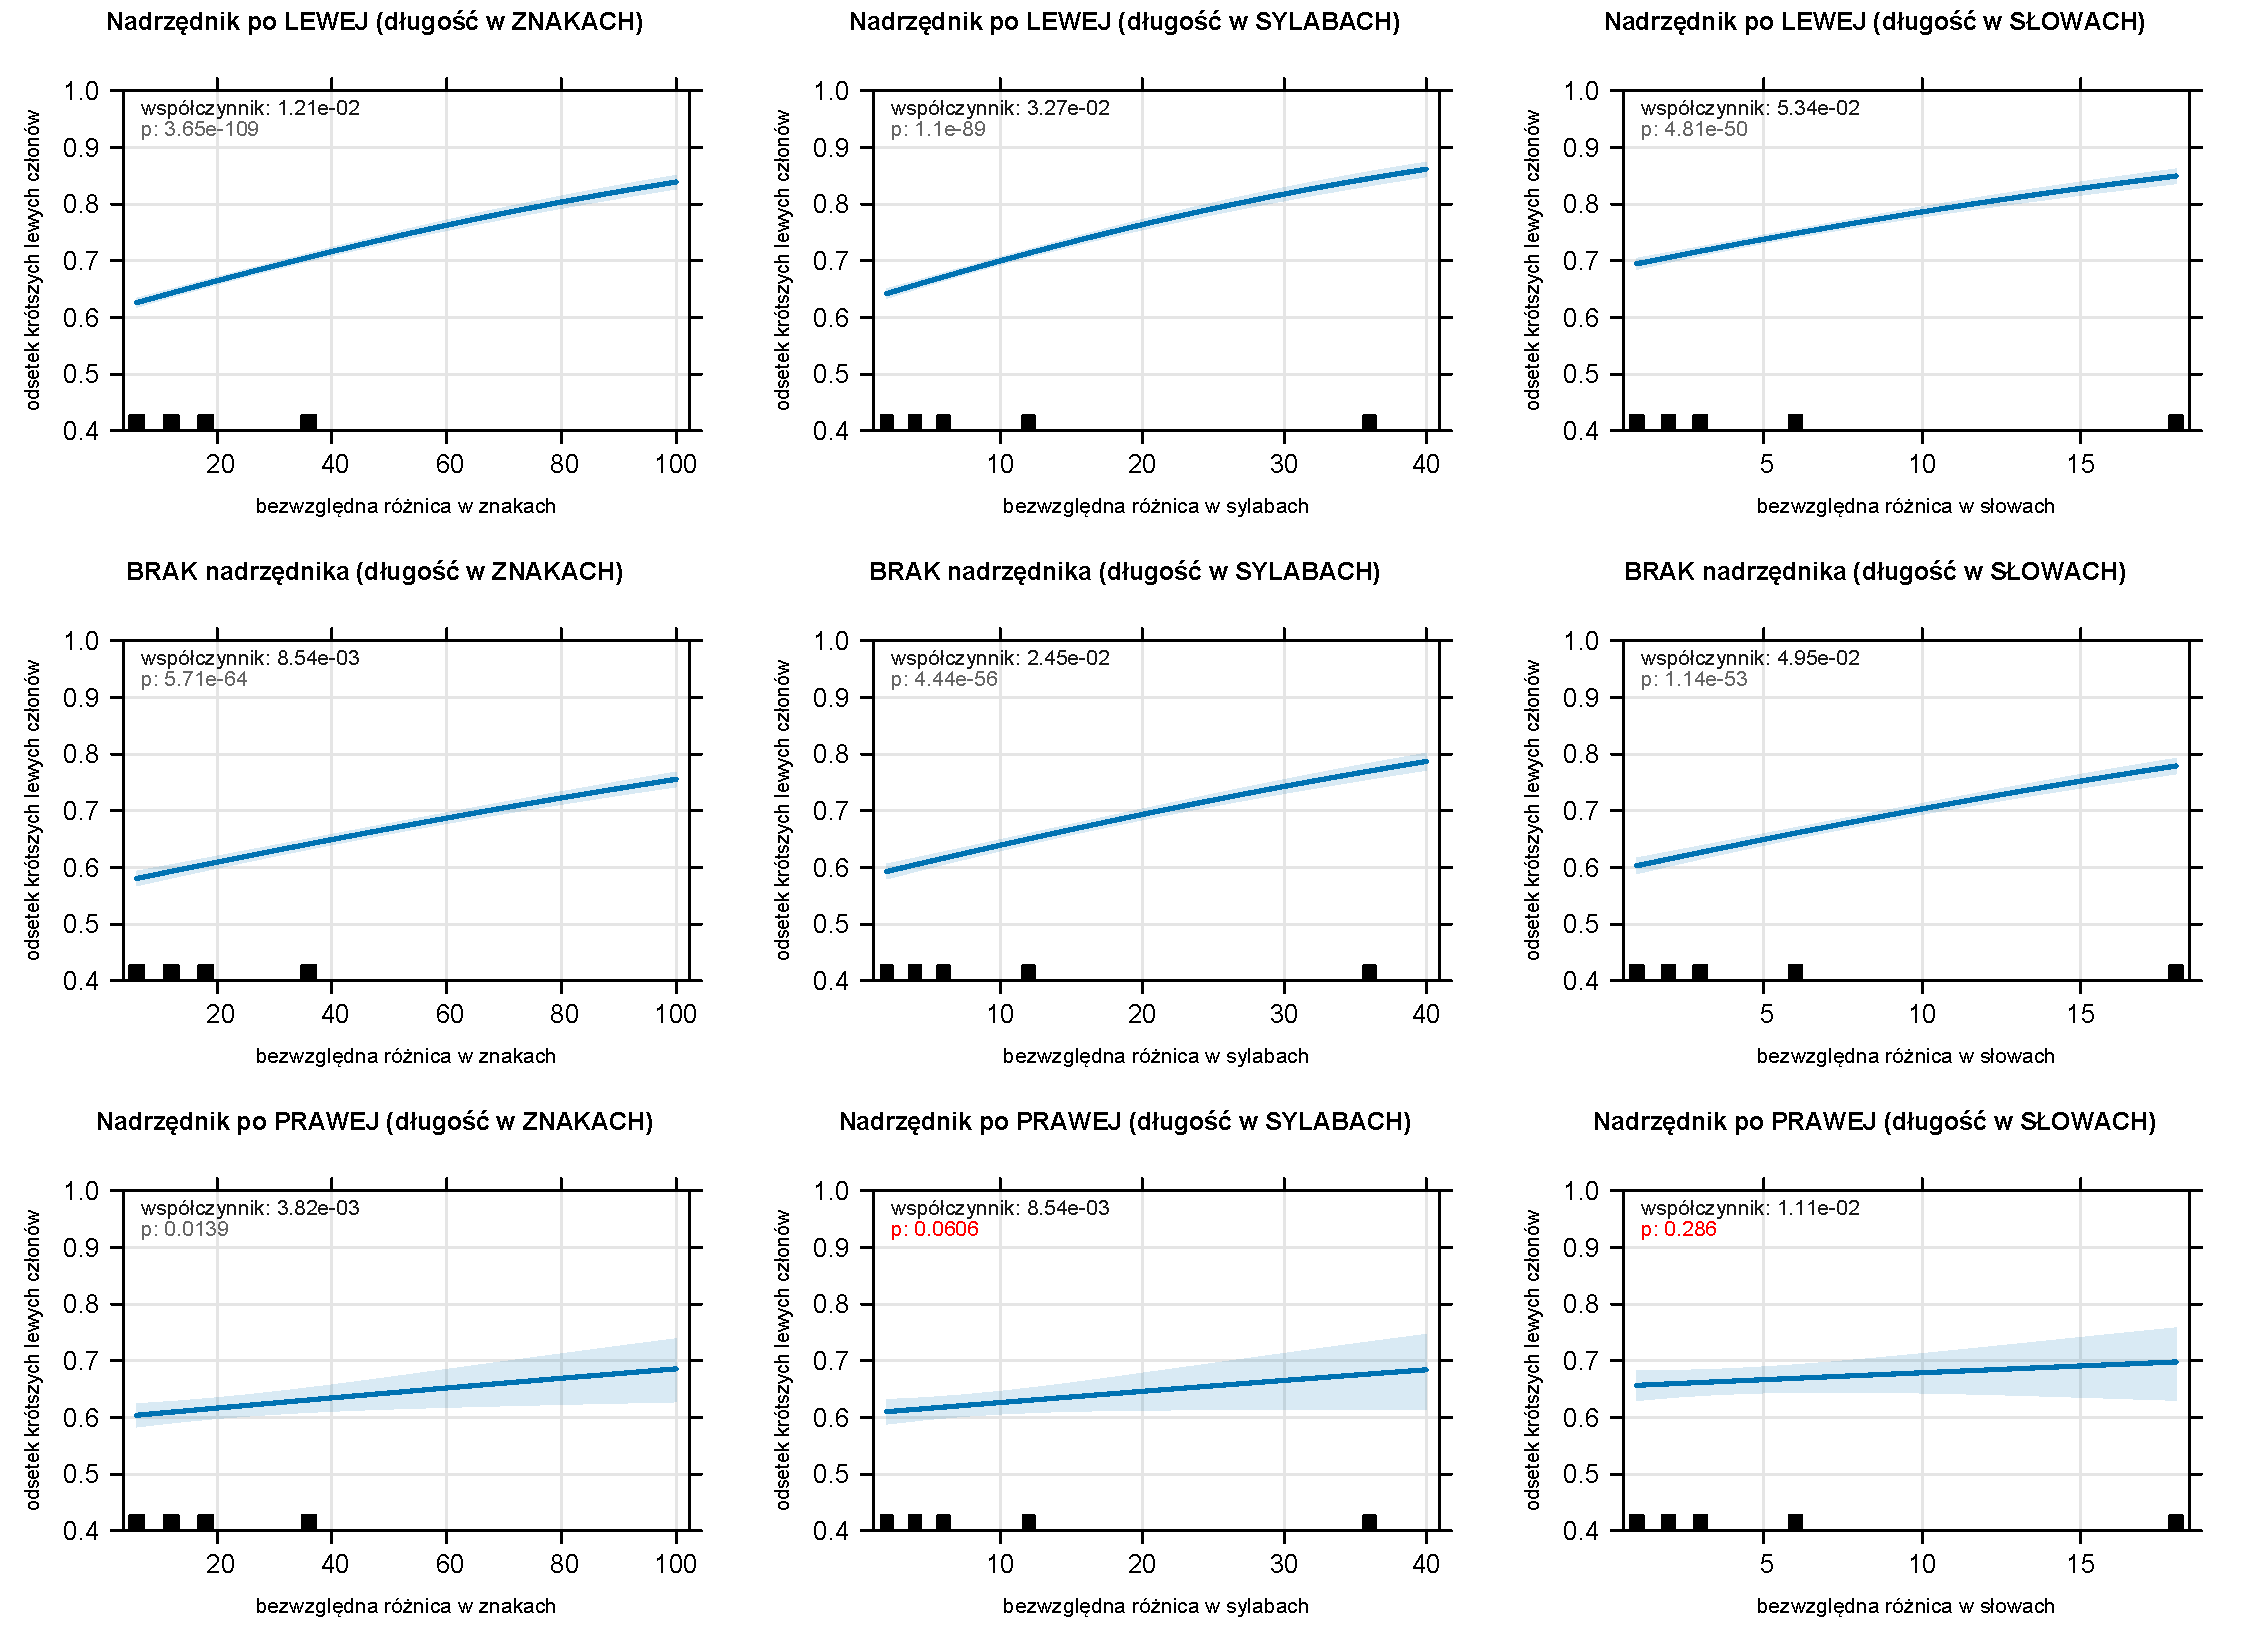
\includegraphics[scale=0.6]{Romanian.pdf}
\caption{Różnica długości członów a występowanie krótszego członu po lewej stronie -- język \textbf{rumuński}}
\label{fig:ro}
\end{sidewaysfigure}

\begin{sidewaysfigure}
\centering
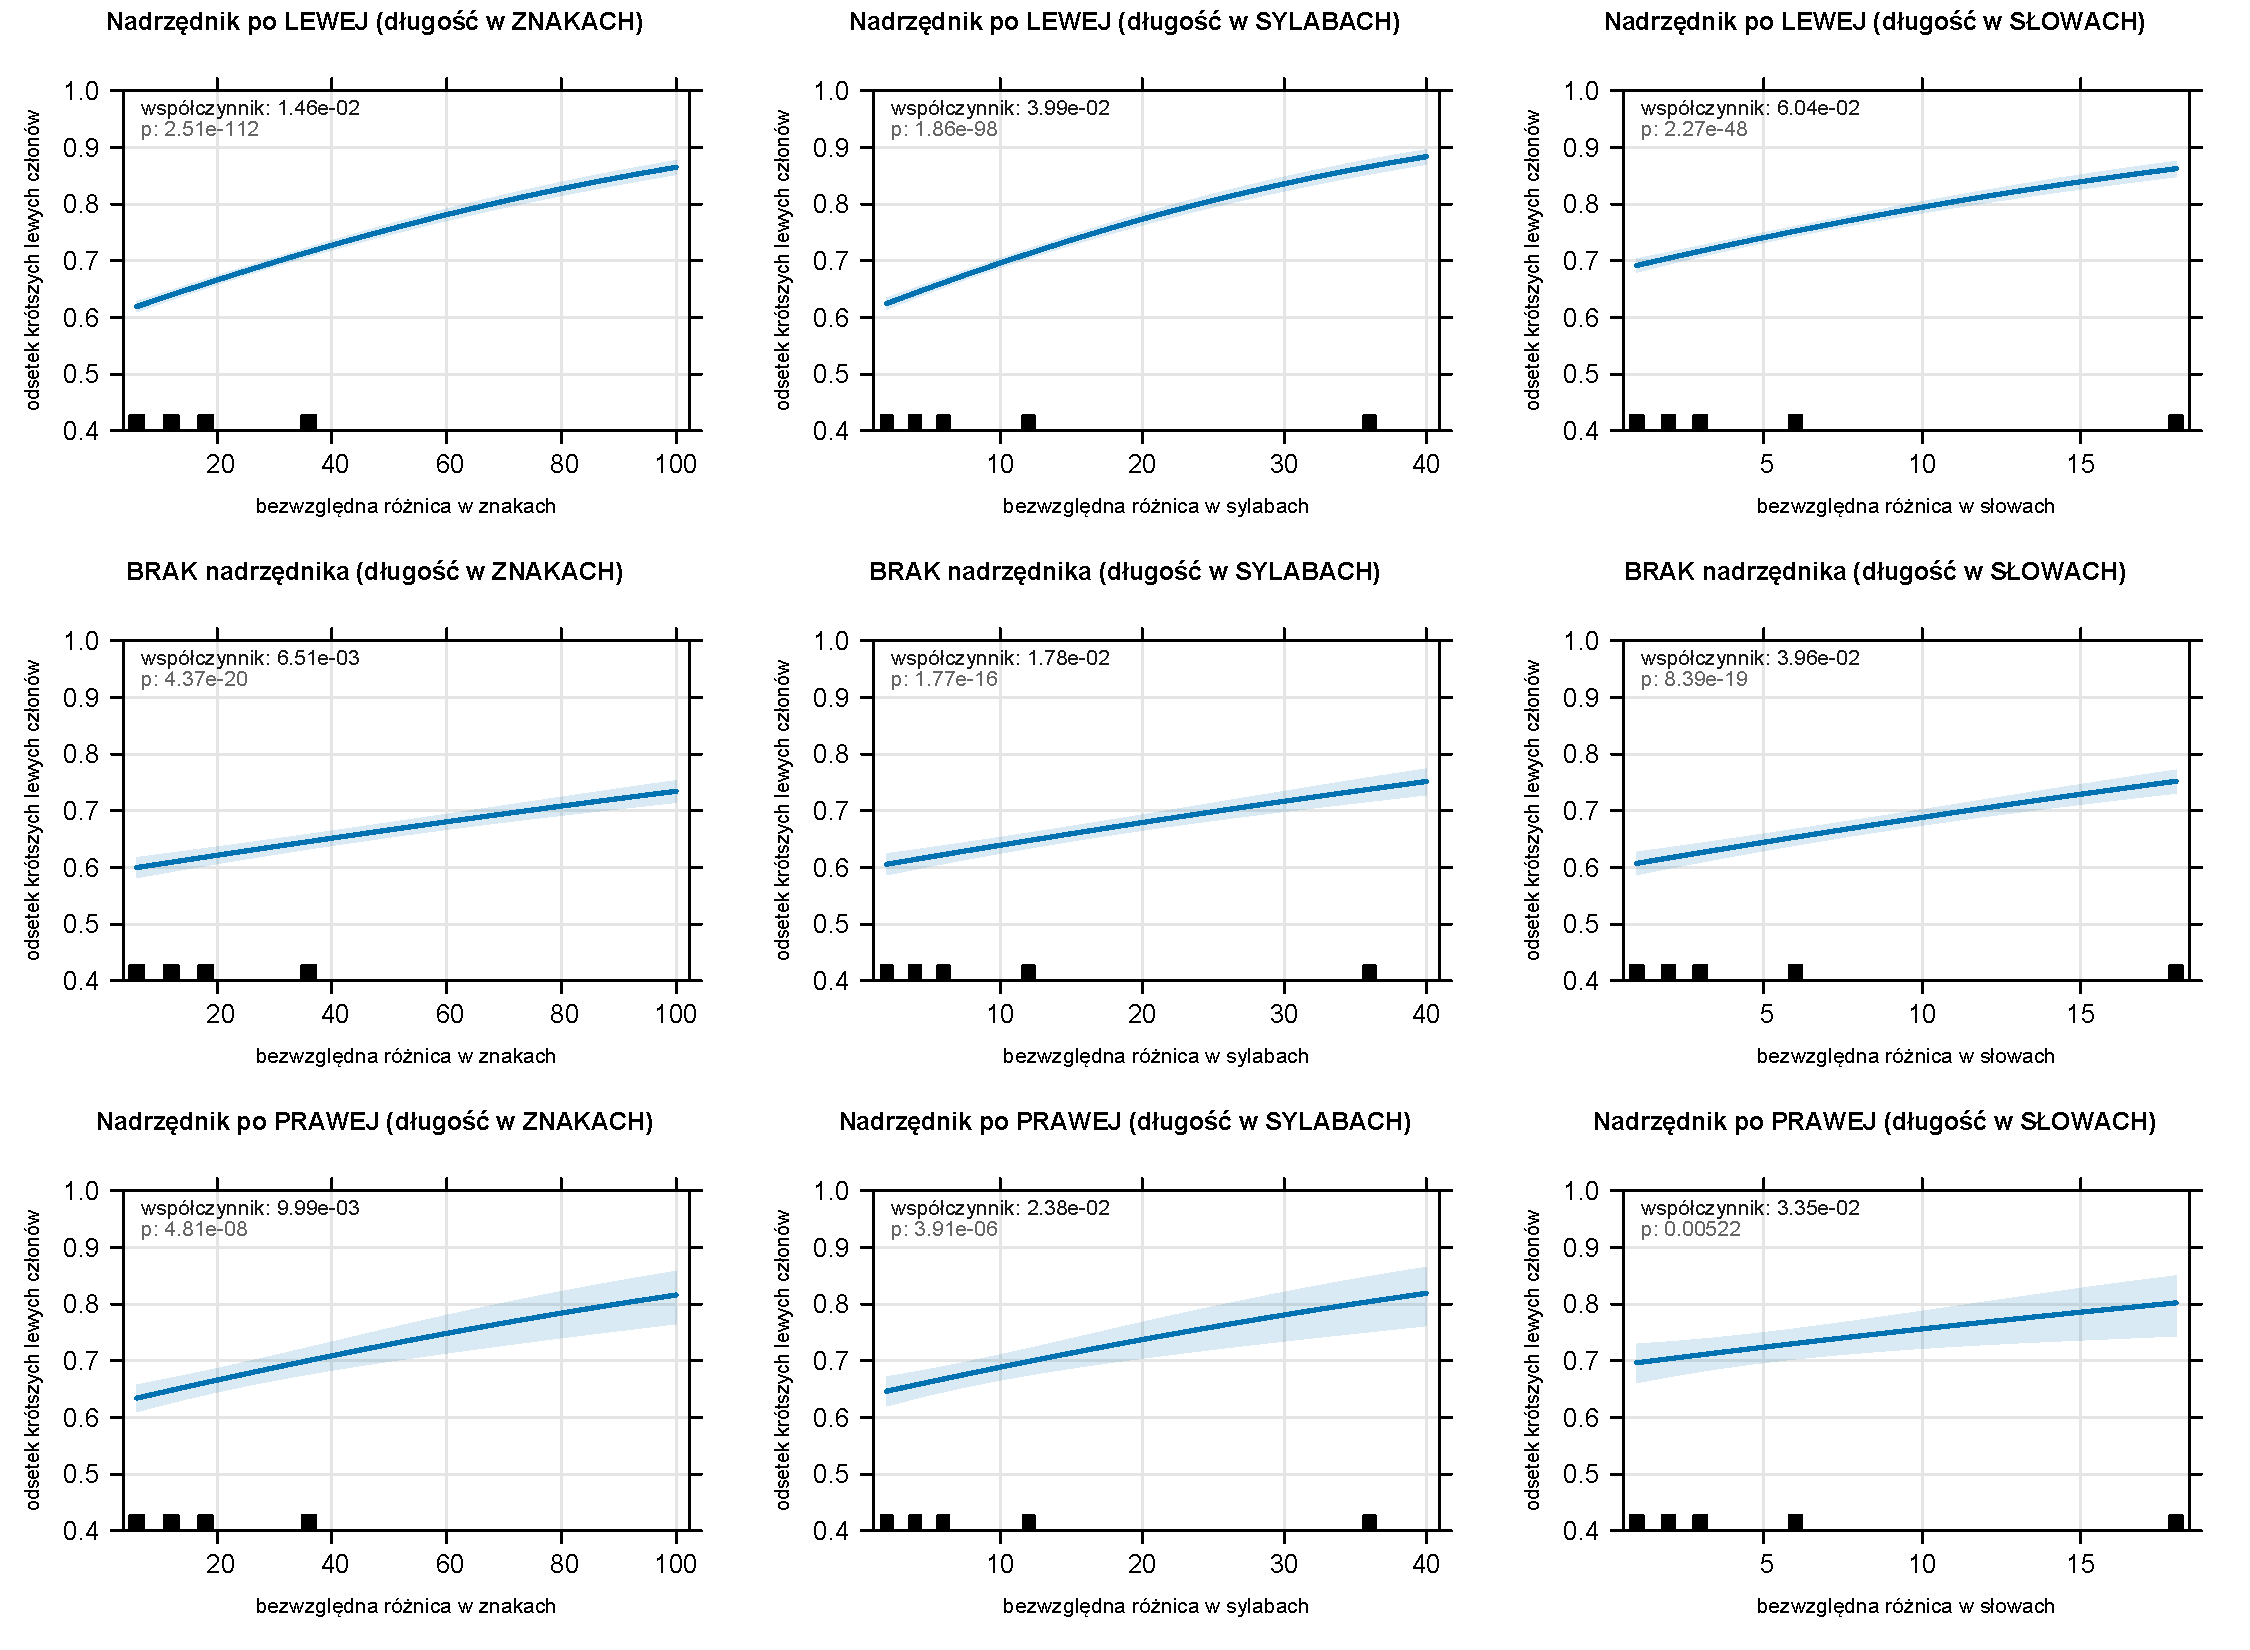
\includegraphics[scale=0.6]{Italian.pdf}
\caption{Różnica długości członów a występowanie krótszego członu po lewej stronie -- język \textbf{włoski}}
\label{fig:it}
\end{sidewaysfigure}

\newpage

\section{Języki mieszane}

\begin{sidewaysfigure}
\centering
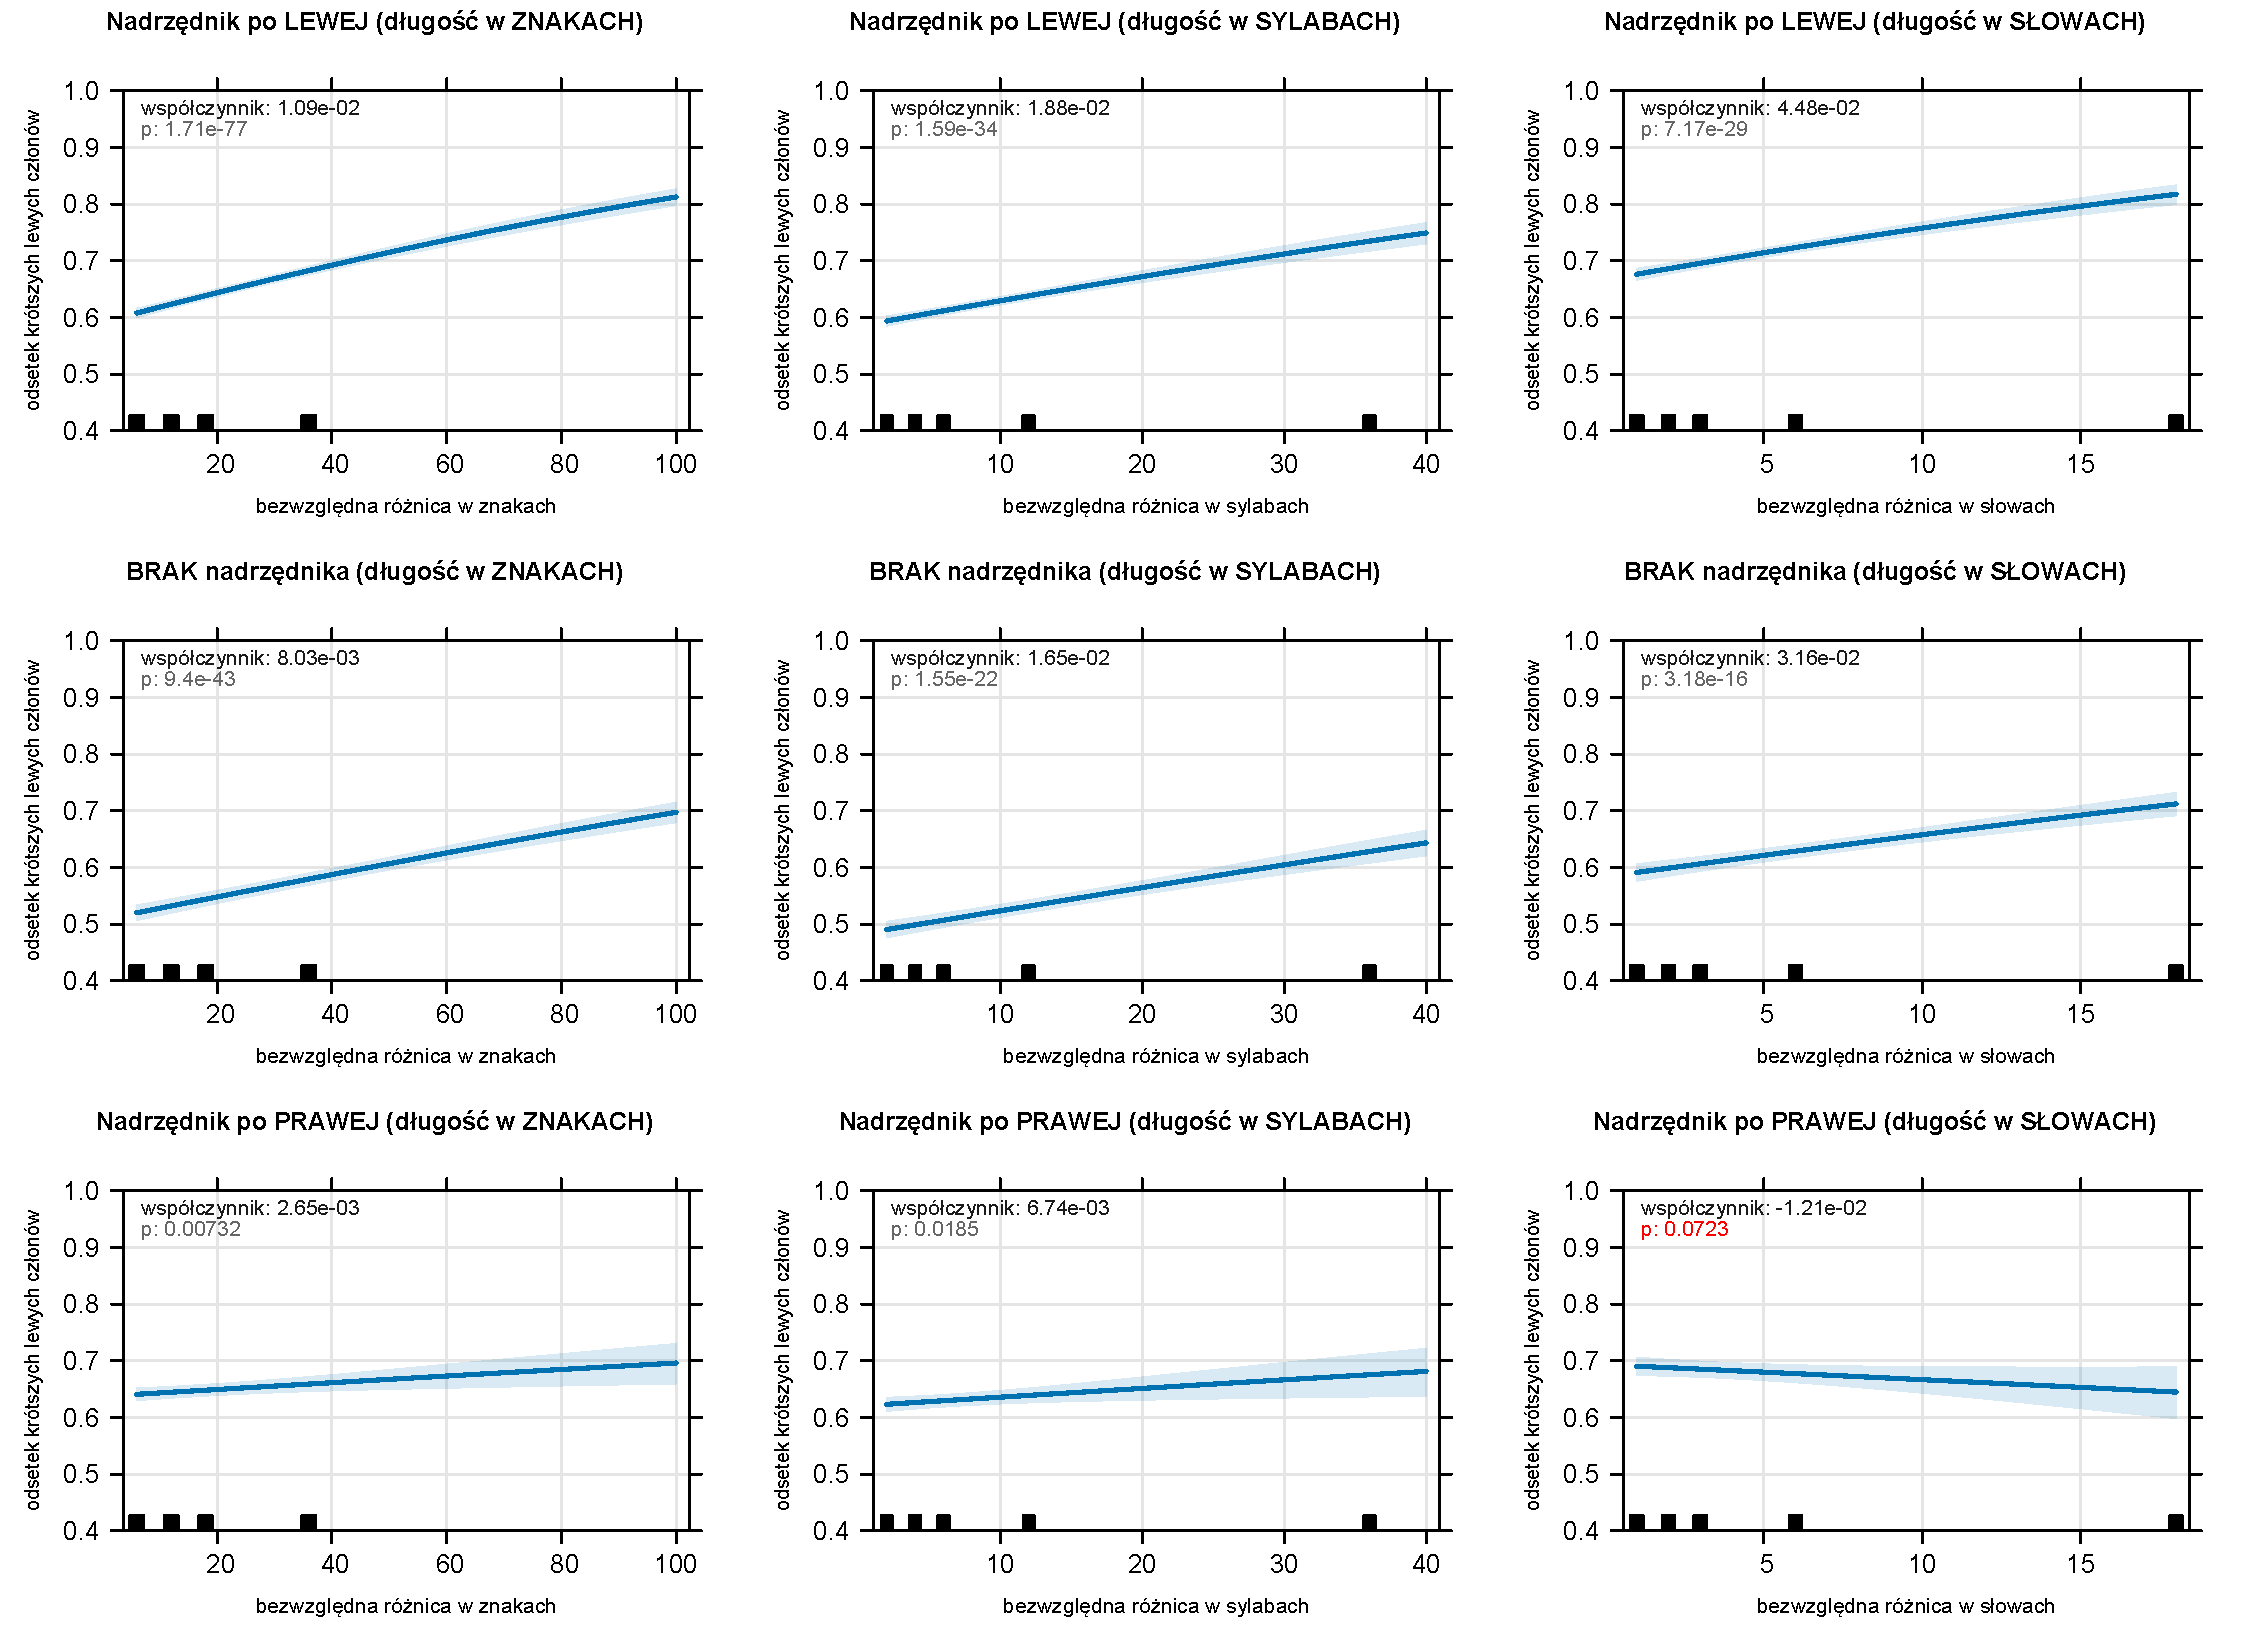
\includegraphics[scale=0.6]{Latin.pdf}
\caption{Różnica długości członów a występowanie krótszego członu po lewej stronie -- język \textbf{łaciński}}
\label{fig:la}
\end{sidewaysfigure}

\begin{sidewaysfigure}
\centering
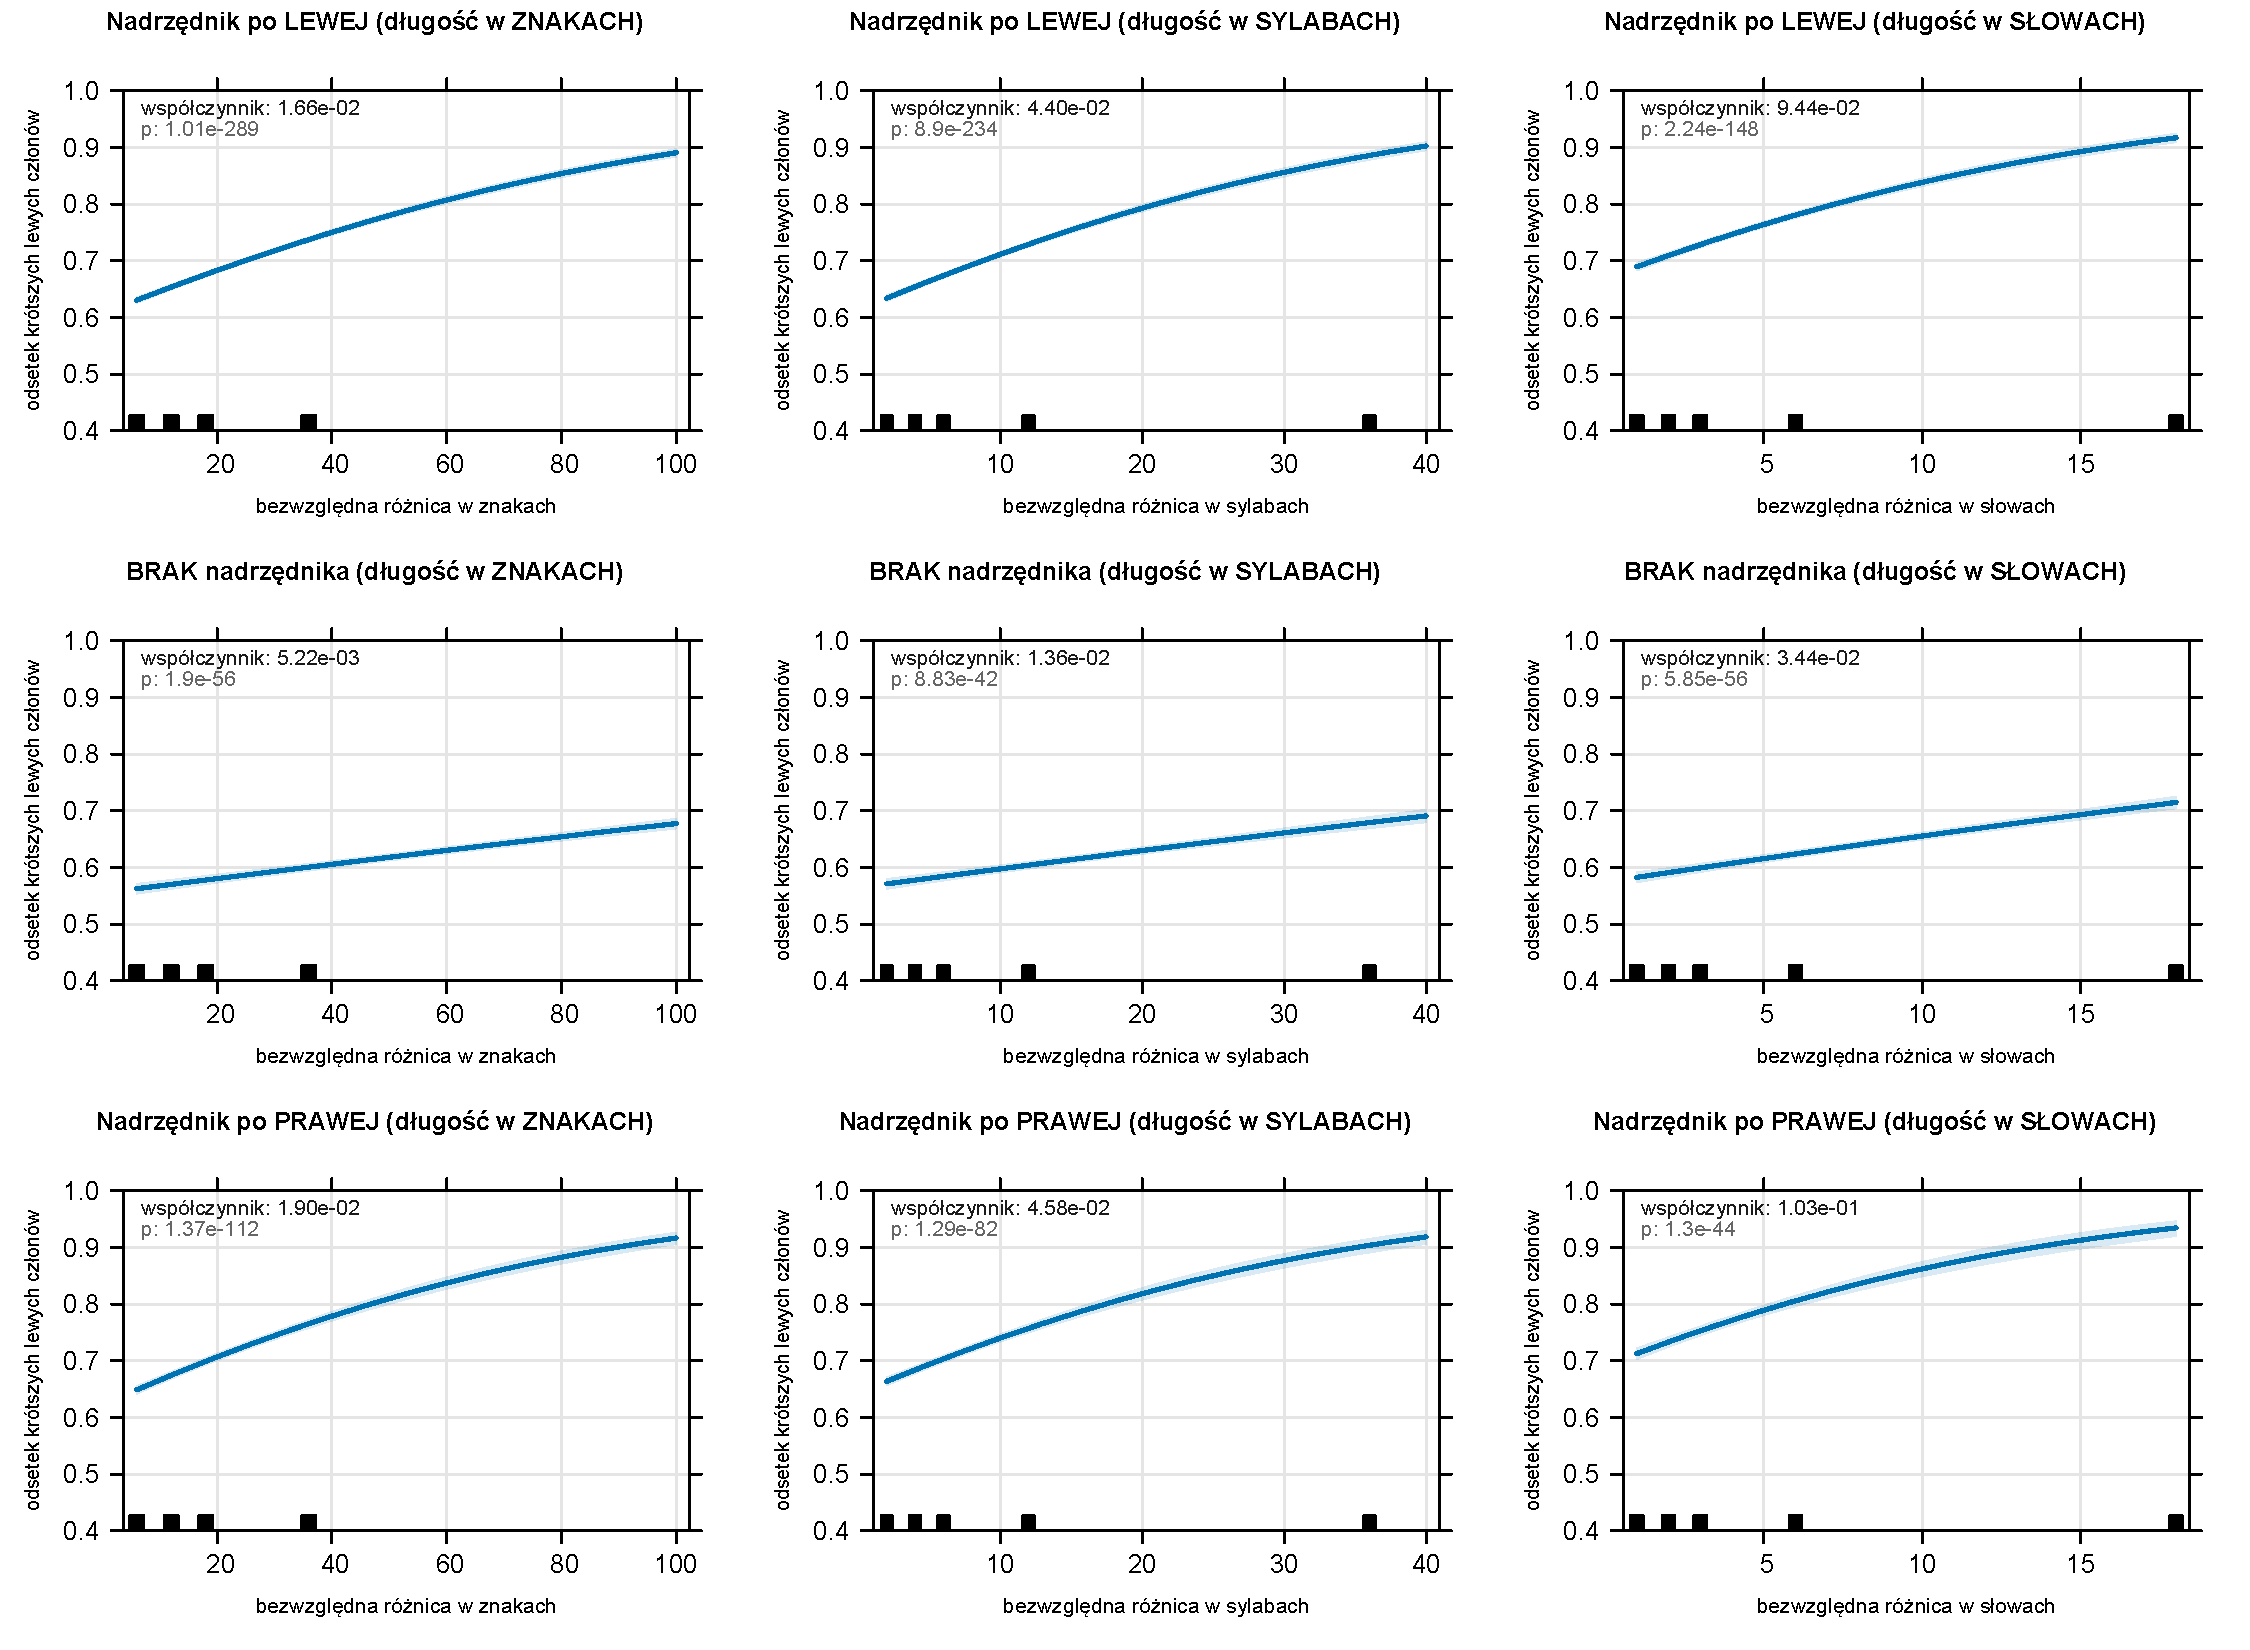
\includegraphics[scale=0.6]{German.pdf}
\caption{Różnica długości członów a występowanie krótszego członu po lewej stronie -- język \textbf{niemiecki}}
\label{fig:de}
\end{sidewaysfigure}

\newpage

\section{Języki finalne}

\begin{sidewaysfigure}
\centering
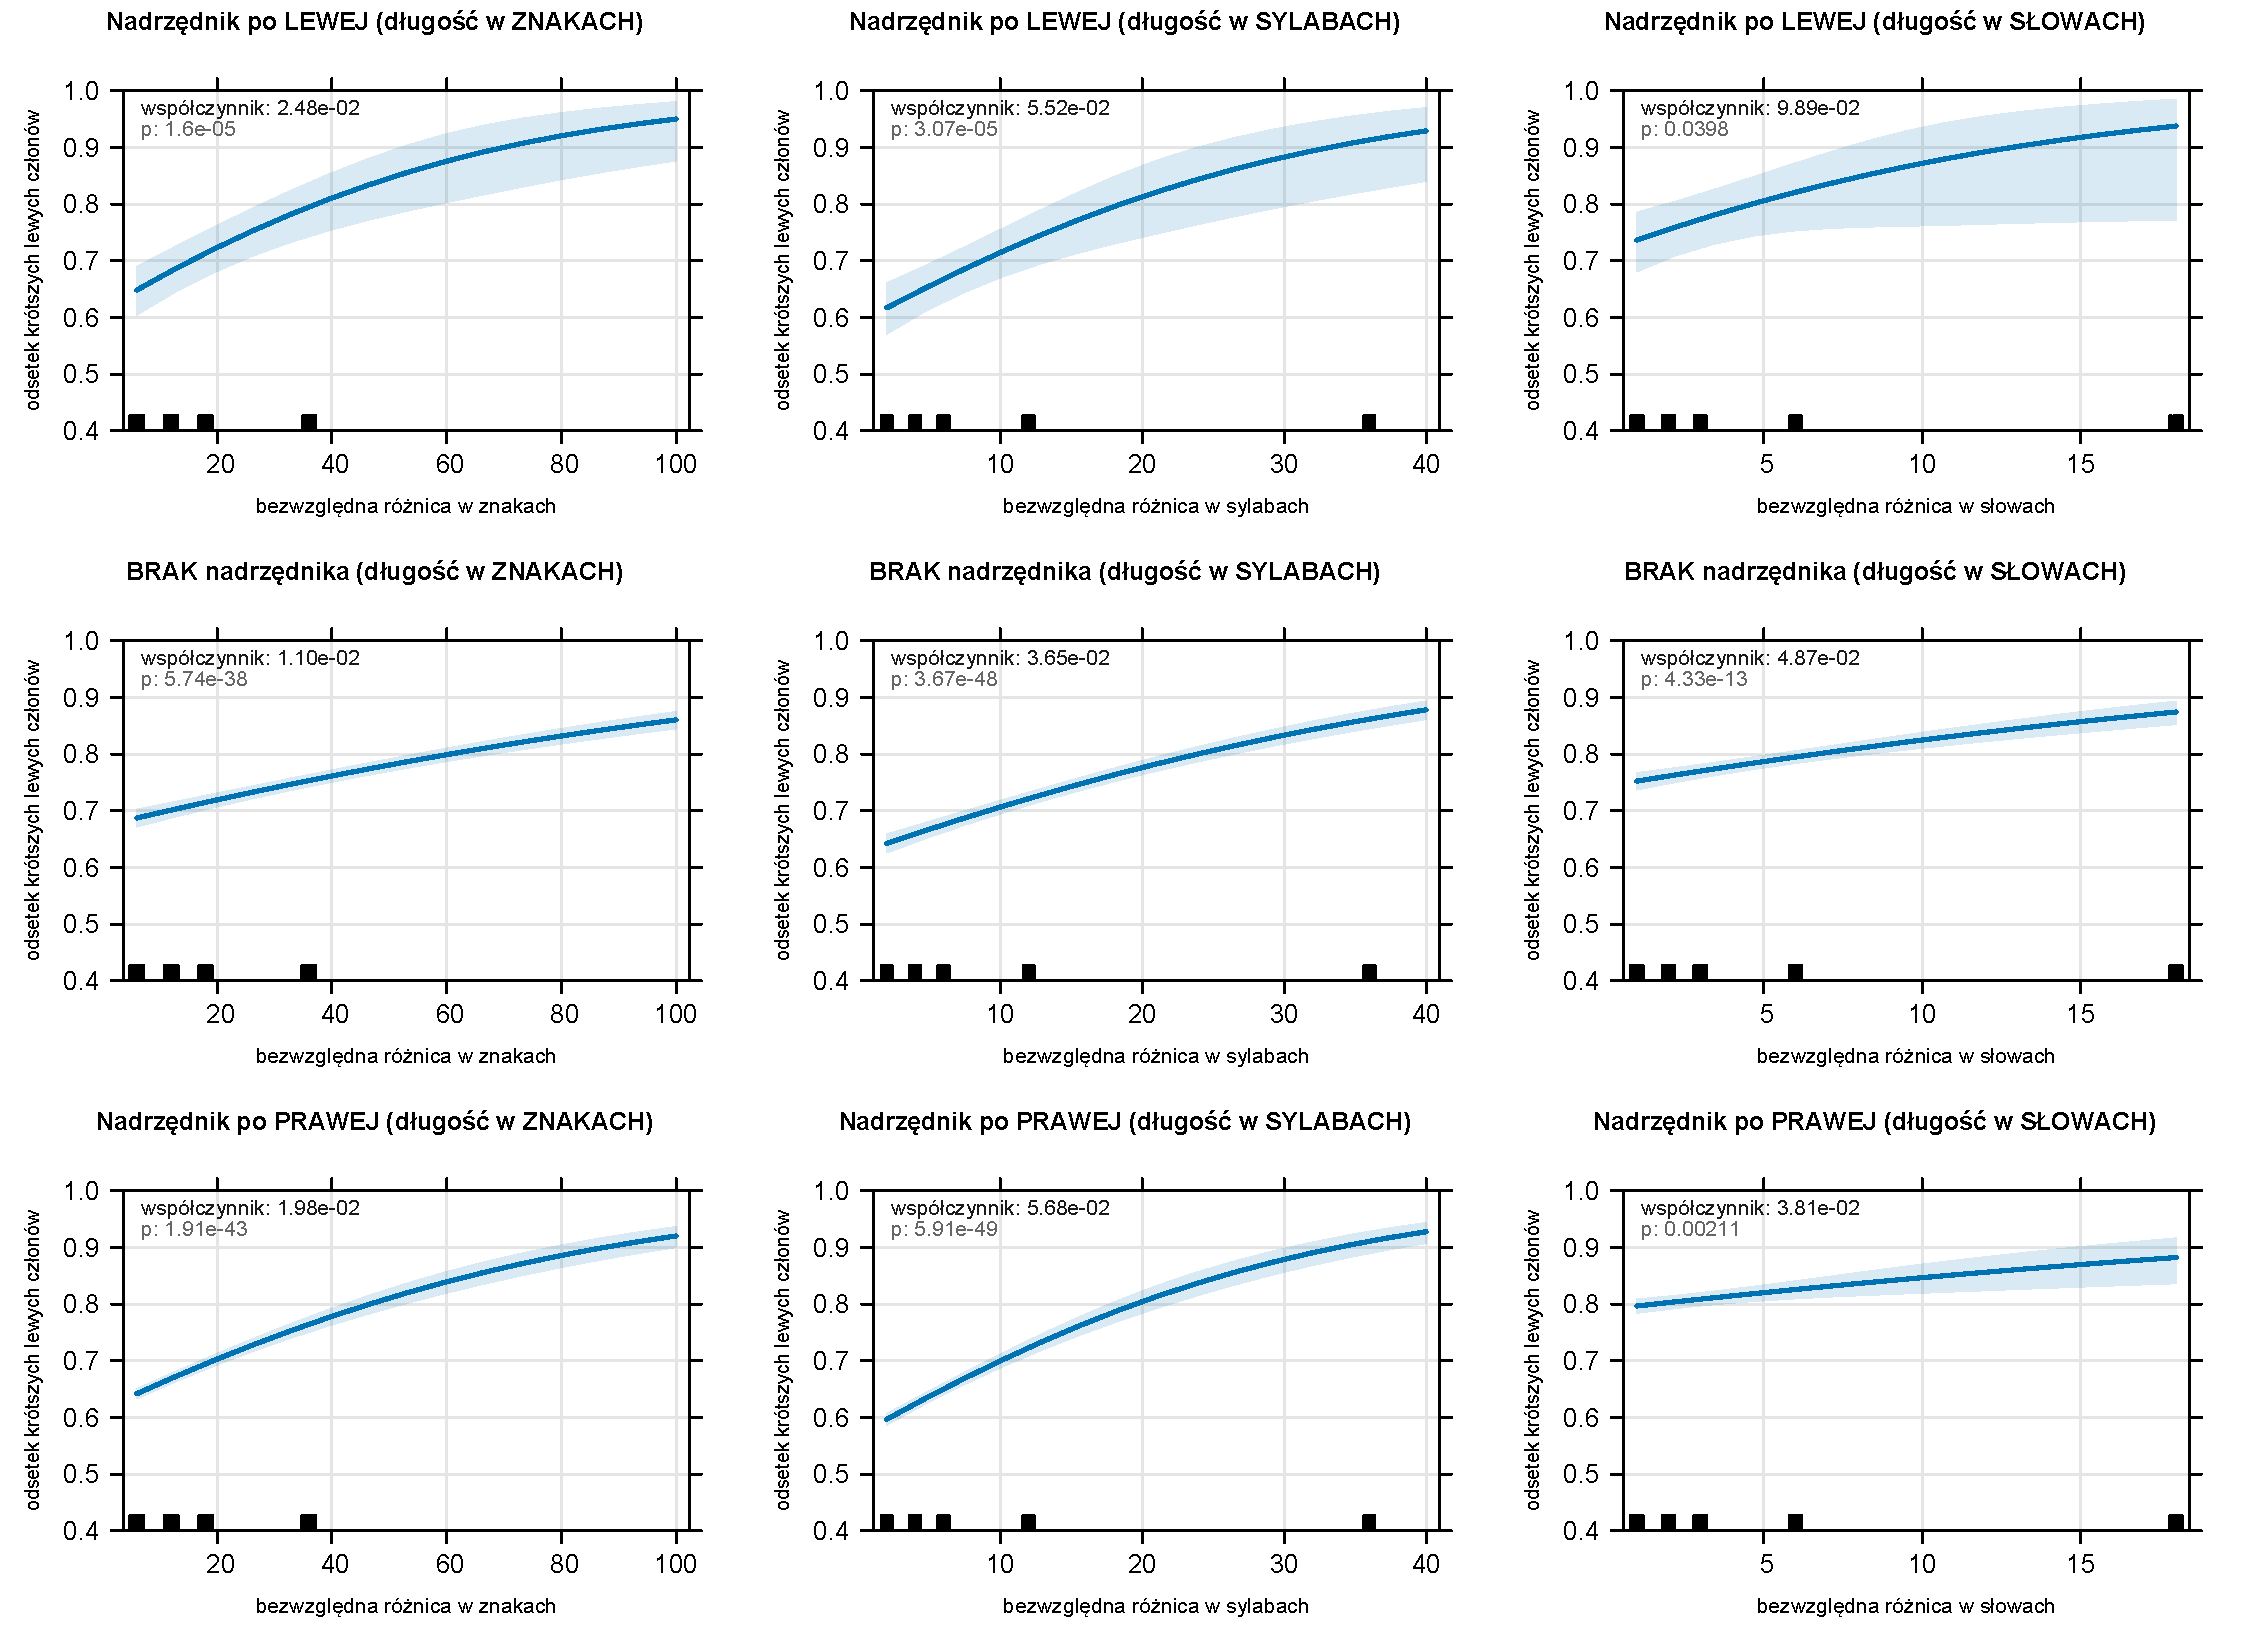
\includegraphics[scale=0.6]{Korean.pdf}
\caption{Różnica długości członów a występowanie krótszego członu po lewej stronie -- język \textbf{koreański}}
\label{fig:ko}
\end{sidewaysfigure}

\begin{sidewaysfigure}
\centering
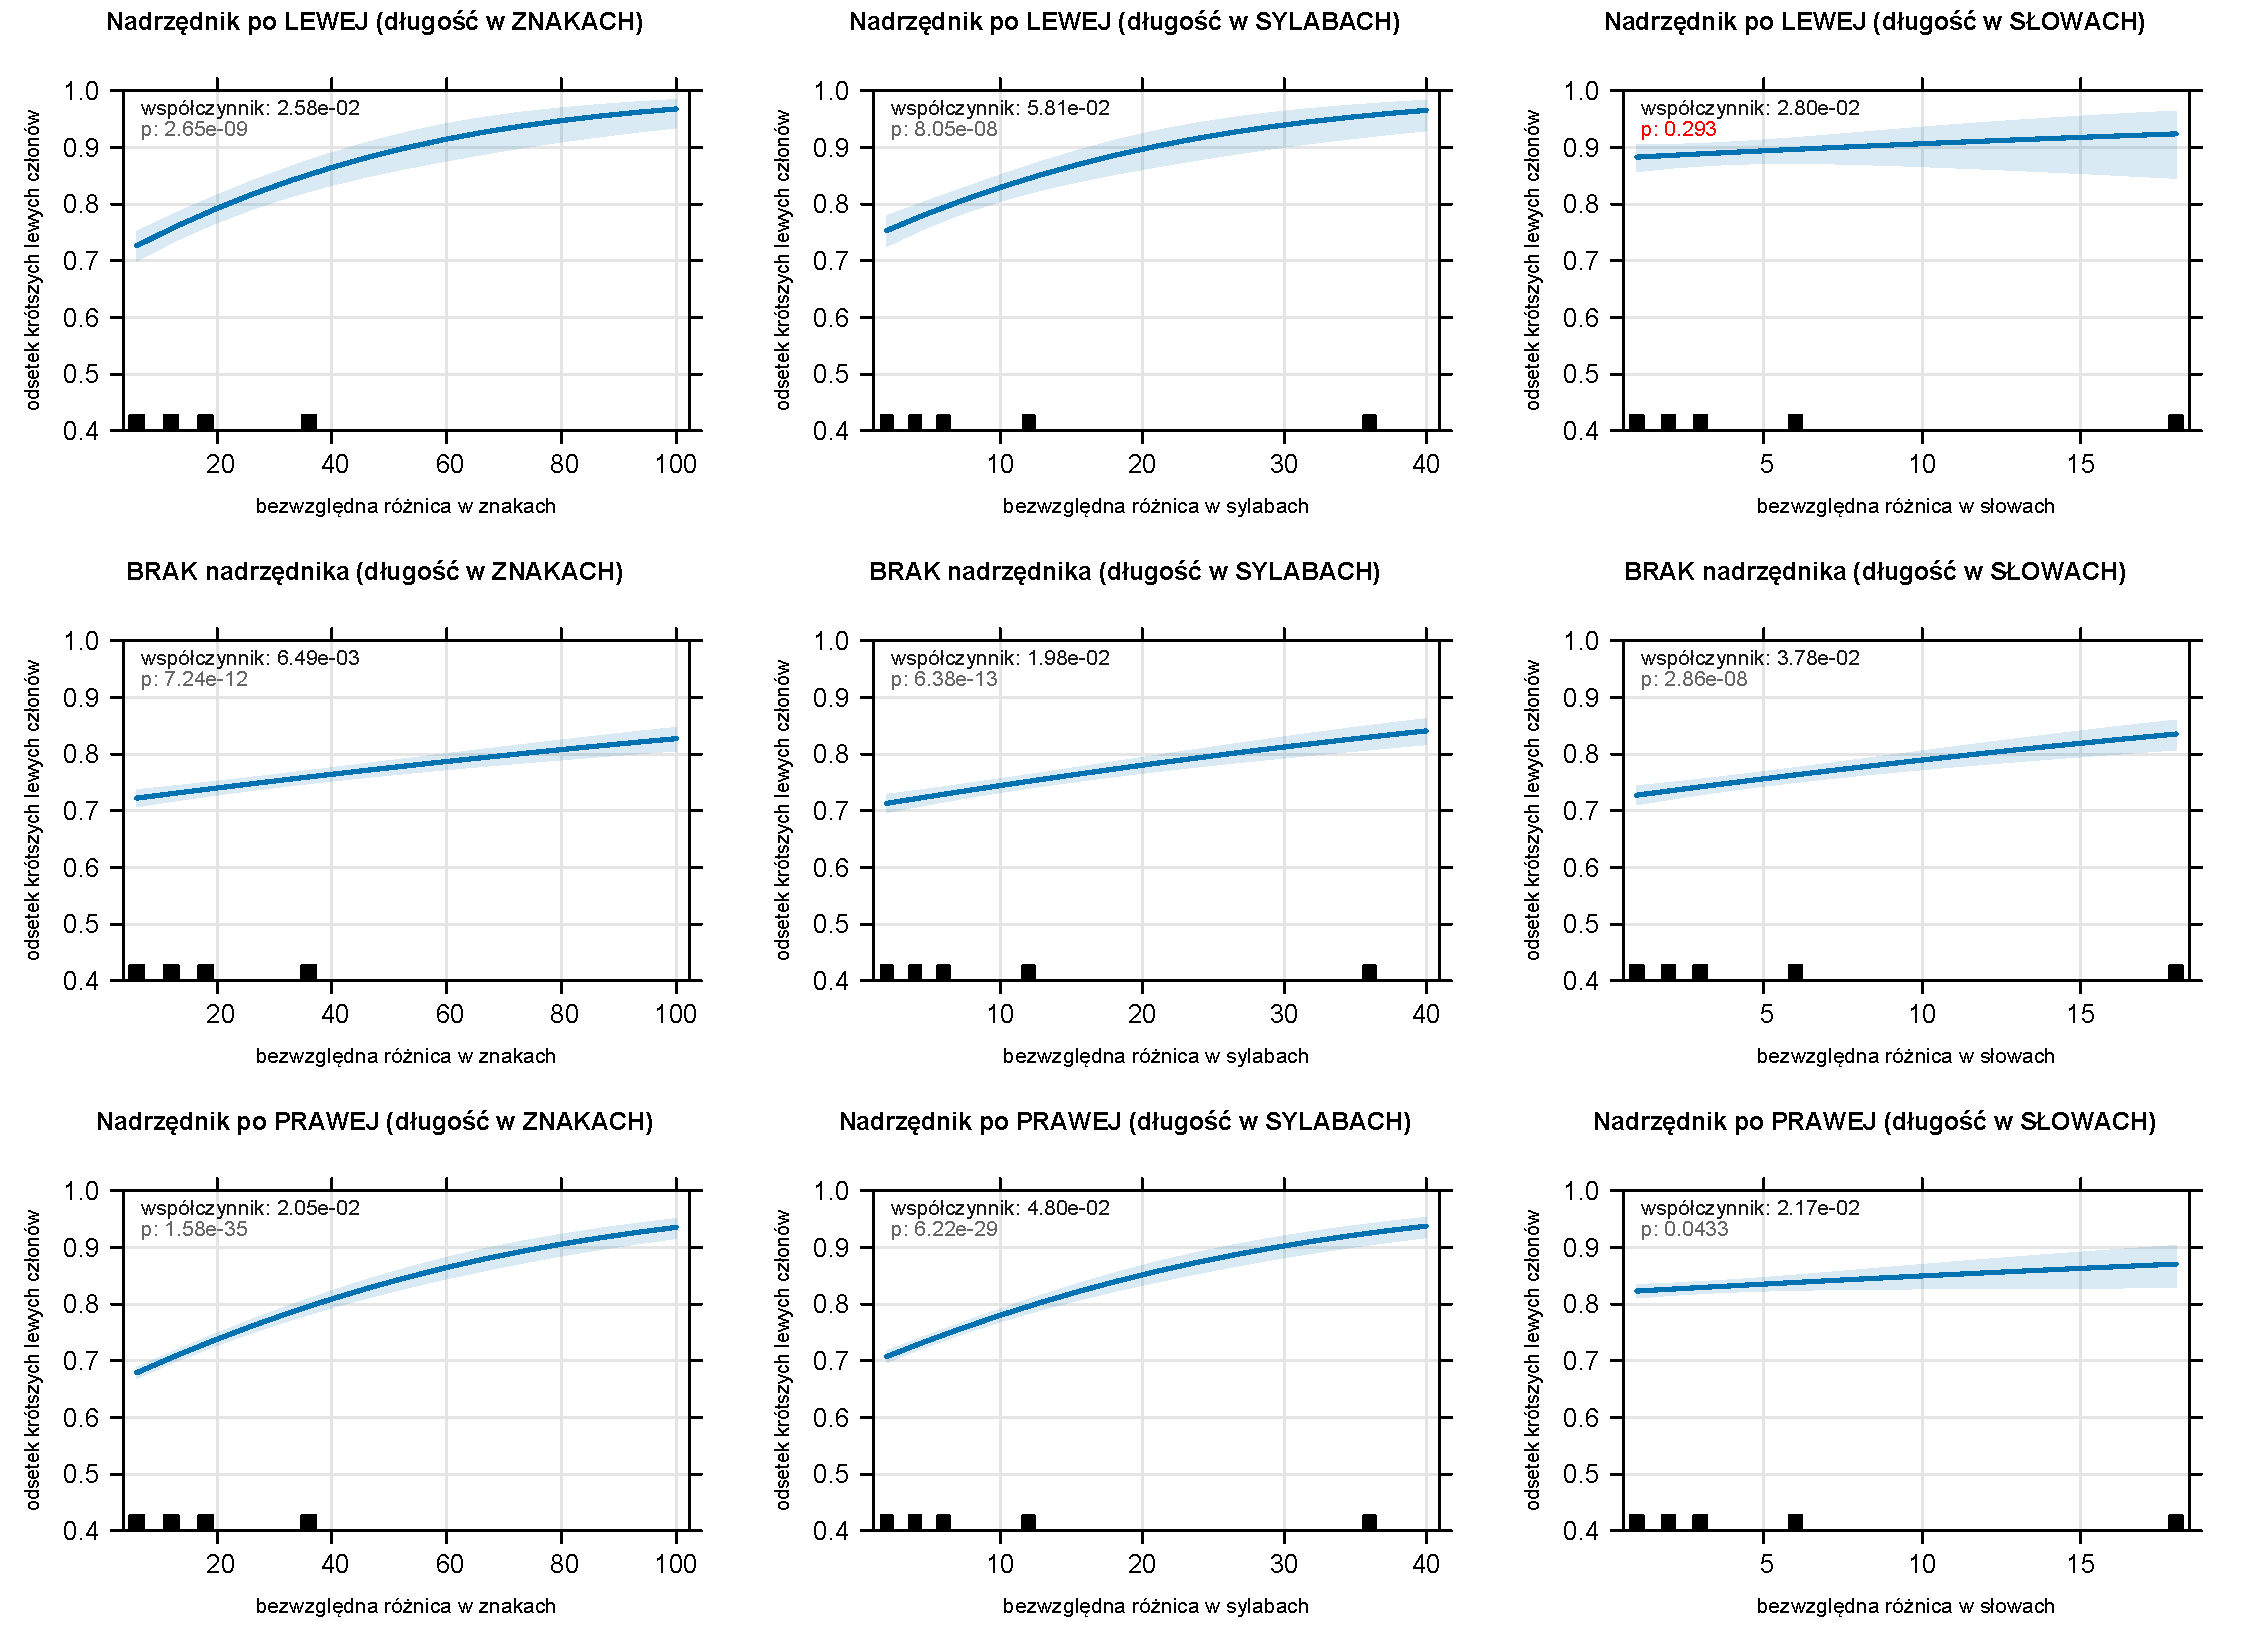
\includegraphics[scale=0.6]{Turkish.pdf}
\caption{Różnica długości członów a występowanie krótszego członu po lewej stronie -- język \textbf{turecki}}
\label{fig:tr}
\end{sidewaysfigure}